% -- Anfang Präambel
\documentclass[german,  % Standardmäßig deutsche Eigenarten, englisch -> english
parskip=full,  % Absätze durch Leerzeile trennen
%bibliography=totoc,  % Literatur im Inhaltsverzeichnis (ist unüblich)
%draft,  % TODO: Entwurfsmodus -> entfernen für endgültige Version
]{scrartcl}
\usepackage[utf8]{inputenc}  % Kodierung der Datei
\usepackage[T1]{fontenc}  % Vollen Umfang der Schriftzeichen
\usepackage[ngerman]{babel}  % Sprache auf Deutsch (neue Rechtschreibung)

% Mathematik und Größen
\usepackage{amsmath}
\usepackage[locale=DE,  % deutsche Eigenarten, englisch -> US
separate-uncertainty,  % Unsicherheiten seperat angeben (mit ±)
]{siunitx}
\usepackage{physics}  % Erstellung von Gleichungen vereinfachen

\usepackage{graphicx}  % Bilder einbinden \includegraphics{Pfad/zur/Datei(ohne Dateiendung)}

% Gestaltung
%\usepackage{microtype}  % Mikrotypographie (kann man am Ende verwenden)
\usepackage{booktabs}  % schönere Tabellen
%\usepackage[toc]{multitoc}  % mehrspaltiges Inhaltsverzeichnis
\usepackage{csquotes}  % Anführungszeichen mit \enquote
\usepackage{caption}  % Anpassung der Bildunterschriften, Tabellenüberschriften
\usepackage{subcaption}  % Unterabbildungen, Untertabellen, …
\usepackage{enumitem}  % Listen anpassen
\setlist{itemsep=-10pt}  % Abstände zwischen Listenpunkten verringern

% Manipulation des Seitenstils
\usepackage{scrpage2}
% Kopf-/Fußzeilen setzen
\pagestyle{scrheadings}  % Stil für die Seite setzen
\clearscrheadings  % Stil zurücksetzen, um ihn neu zu definieren
\automark{section}  % Abschnittsnamen als Seitenbeschriftung verwenden
\ofoot{\pagemark}  % Seitenzahl außen in Fußzeile
\ihead{\headmark}  % Seitenbeschriftung mittig in Kopfzeile
\setheadsepline{.5pt}  % Kopzeile durch Linie abtrennen

\usepackage[hidelinks]{hyperref}  % Links und weitere PDF-Features

% TODO: Titel und Autor, … festlegen
\newcommand*{\titel}{Realstrukturanalyse}
\newcommand*{\autor}{Tom Drechsler, Konstantin Schmid}
\newcommand*{\abk}{RA}
\newcommand*{\betreuer}{Rolf Schaarschuch}
\newcommand*{\messung}{29. November 2019}
\newcommand*{\ort}{REC/B02}

\hypersetup{pdfauthor={\autor}, pdftitle={\titel}}  % PDF-Metadaten setzen




% Subsubsubsection erzeugen
%\usepackage{titlesec}
%\usepackage{hyperref}

%\titleclass{\subsubsubsection}{straight}[\subsection]

%\newcounter{subsubsubsection}[subsubsection]
%\renewcommand\thesubsubsubsection{\thesubsubsection.\arabic{subsubsubsection}}
%\renewcommand\theparagraph{\thesubsubsubsection.\arabic{paragraph}} % optional; useful if paragraphs are to be numbered

%\titleformat{\subsubsubsection}
  %{\normalfont\normalsize\bfseries}{\thesubsubsubsection}{1em}{}
%\titlespacing*{\subsubsubsection}
%{0pt}{3.25ex plus 1ex minus .2ex}{1.5ex plus .2ex}

%\makeatletter
%\renewcommand\paragraph{\@startsection{paragraph}{5}{\z@}%
  %{3.25ex \@plus1ex \@minus.2ex}%
  %{-1em}%
  %{\normalfont\normalsize\bfseries}}
%\renewcommand\subparagraph{\@startsection{subparagraph}{6}{\parindent}%
  %{3.25ex \@plus1ex \@minus .2ex}%
  %{-1em}%
  %{\normalfont\normalsize\bfseries}}
%\def\toclevel@subsubsubsection{4}
%\def\toclevel@paragraph{5}
%\def\toclevel@paragraph{6}
%\def\l@subsubsubsection{\@dottedtocline{4}{7em}{4em}}
%\def\l@paragraph{\@dottedtocline{5}{10em}{5em}}
%\def\l@subparagraph{\@dottedtocline{6}{14em}{6em}}
%\makeatother

%\setcounter{secnumdepth}{4}
%\setcounter{tocdepth}{4}

\addto{\captionsngerman}{
\renewcommand*{\figurename}{Abb.}
}




% automatischen Titel konfigurieren
\titlehead{F-Praktikum \abk \hfill TU Dresden}
%\subject{Interferometer}
\title{\titel}
\author{\autor}
\date{\begin{tabular}{ll}
Protokoll: & \today\\
Messung: & \messung\\
Ort: & \ort\\
Betreuer: & \betreuer\end{tabular}}

% -- Ende Präambel

\begin{document}
\begin{titlepage}
\maketitle  % Titel setzen
\tableofcontents  % Inhaltsverzeichnis setzen
\end{titlepage}

\section{Ziel und Versuchsprinzip}
Wenn man an ein Kristallgitter denkt, stellt man sich normalerweise zuerst ein streng periodisches Kristallgitter vor. Jedoch gibt es in der Realität stets Abweichungen von dieser idealen Struktur. Diese sollen in diesem Versuch beispielhaft für Silizium untersucht werden. Dazu wird ein Siliziumkristall geläppt, anschließend angeäzt und unter dem Mikroskop betrachtet. Im zweiten Versuchsteil soll je ein Zylinder aus Messing und Stahl geschliffen, poliert, angeäzt und unter dem Mikroskop betrachtet werden. Die so entstandenen Aufnahmen werden sterographisch untersucht. So können der Anteil von $\alpha$- bzw. $\beta$-Messing, sowie der Kohlenstoffgehalt des Stahls bestimmt werden. Beim Silizium lassen sich durch die Analyse von Ätzgrübchen die Orientierung der untersuchten Kristallebene sowie eine Versetzungsdichte bestimmen.

\section{Theoretische Grundlagen}
\subsection{Gitterdefekte}
Gitterdefekte beschreiben die Abweichungen von dem idealen, periodischen Kristallgitter. Diese werden aufgrund ihrer Dimensionalität in 4 Gruppen eingeteilt:
\begin{itemize}
\item Punktdefekte (0-dimensional): Leerstellen, Zwischengitteratome, Substitutionsatome
\item Linienfehler (1-dimensional): Stufenversetzungen, Schraubenversetzungen
\item Flächenfehler (2-dimensional): Stapelfehler, Klein- und Großwinkelkorngrenzen, Zwillingskorngrenzen
\item Volumenfehler (3-dimensional): Poren, Einschlüsse
\end{itemize}
In diesem Versuch werden vor allem Stufenversetzungen und Klein- bzw. Großwinkelkorngrenzen wichtig werden. Deshalb sind diese im Folgenden nochmals erläutert.
\subsubsection{Stufenversetzungen}
Bei einer Stufenversetzung gibt es eine zusätzliche Halbebene, die in die ideale Kristallstruktur eingebracht wird. Dies kann während des Kristallwachstums oder in Folge plastischer Verformung geschehen. Durch diese zusätzliche Halbebene entsteht eine zusätzliche Druckspannung auf den sogenannten Versetzungskern. In Folge dessen ist dort die Bindung innerhalb des Kristalls schwächer. \\\\
\begin{minipage}{0.35 \textwidth} \centering
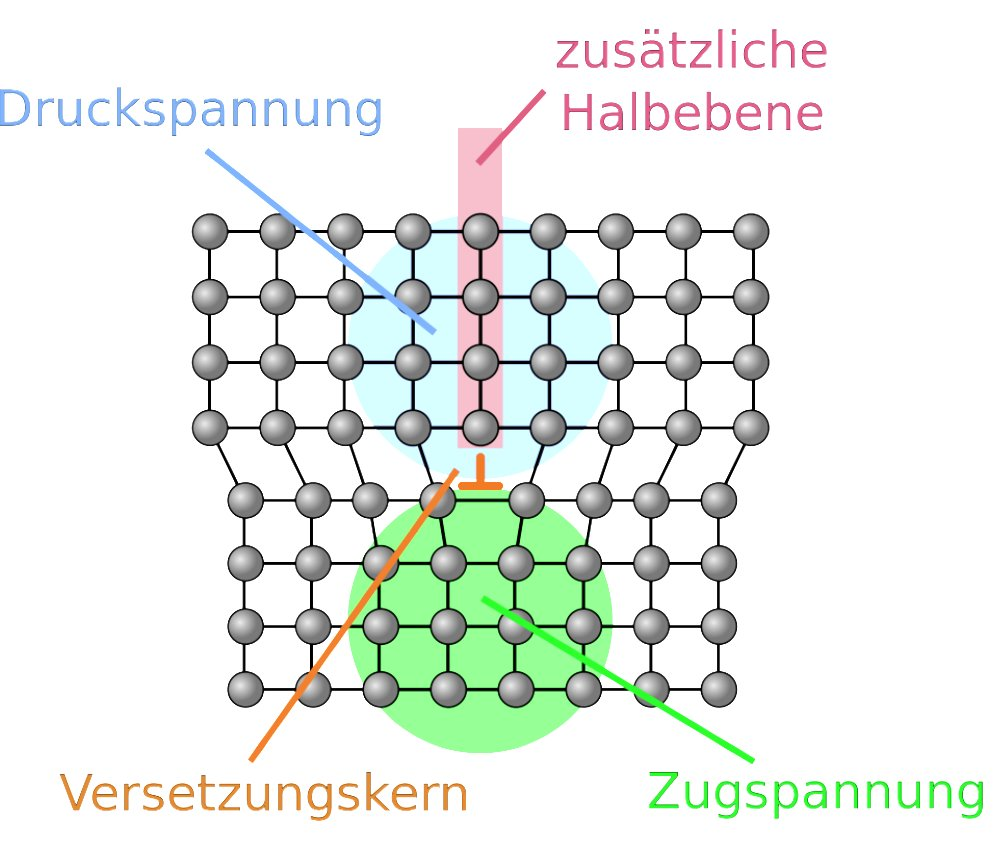
\includegraphics[scale=0.2]{Stufenversetzung1.jpg}
\captionof{figure}{Schematische Darstellung von Stufenversetzungen (2D)}
\end{minipage}
\begin{minipage}{0.2\textwidth}\centering
\[\]
\end{minipage}
\begin{minipage}{0.45 \textwidth} \centering
\[\]
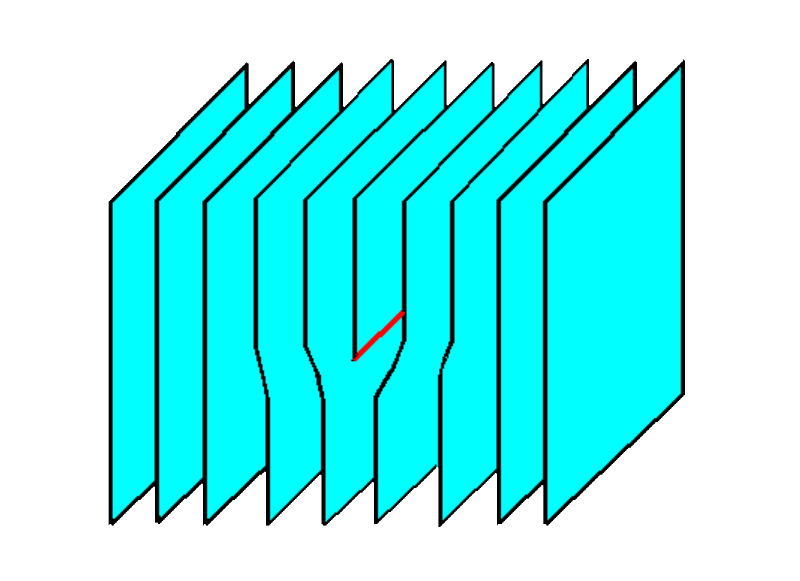
\includegraphics[scale=0.3]{Stufenversetzung2.png}
\captionof{figure}{Schematische Darstellung von Stufenversetzungen (3D)}
\end{minipage}
\\\\\\
Für die mathematische Beschreibung von Stufenversetzungen gibt es eine sehr nützliche Hilfsgröße, nämlich den \textsc{Burgers}-Vektor \(\vec{b}\). Dieser lässt sich wie folgt konstruieren:
\begin{enumerate}
\item Man legt in genügend großer Entfernung zum Versetzungskern eine geschlossene Kette aus Gittervektoren um den Versetzungskern herum.
\item Anschließend betrachtet man das ideale Gitter ohne Versetzungskern und legt wieder eine geschlossene Kette mit derselben Zahl an Gittervektoren pro Seite hinein.
\item Es ergibt sich dann stets genau eine Stelle, an der der Umlauf nicht geschlossen ist, sich aber durch Hinzunahme eines weiteren Gittervektors schließen lässt. Dieser zusätzliche Vektor ist der Burgers-Vektor.
\end{enumerate}
Die nachfolgende Abbildung illustriert den Konstruktionsprozess Schritt für Schritt: 
\newpage
\begin{figure}[h!]\centering
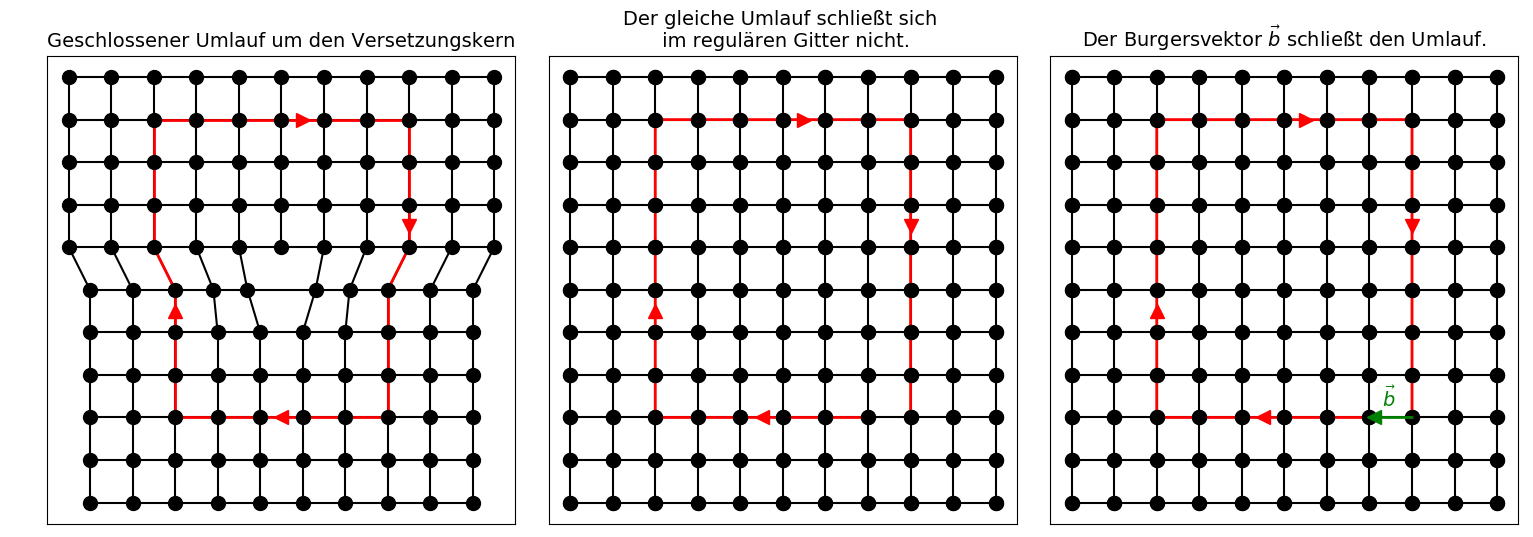
\includegraphics[width=\textwidth]{Burgers_Vektor.png}
\caption{Darstellung der Konstruktion des Burgers-Vektors}
\end{figure}

\subsubsection{Klein-und Großwinkelkorngrenzen}

Eine Anwendung des Burgers-Vektors ist die quantitative Beschreibung von Korngrenzen: 
Beim Wachstum von Kristallen kann es zu Bereichen kommen, in denen einkristalline Bereiche leicht zueinander verkippte Gitterebenen haben. Dies bezeichnet man dann je nach Größe des eingeschlossenen Winkels $\Theta$ als Klein- bzw. Großwinkelkorngrenze. Dabei bezeichnet man solche mit $\Theta < 5^{\circ}...15^{\circ}$ (je nach verwendeter Quelle) als Kleinwinkelkorngrenze.
\\\\
\begin{figure}[h!]\centering
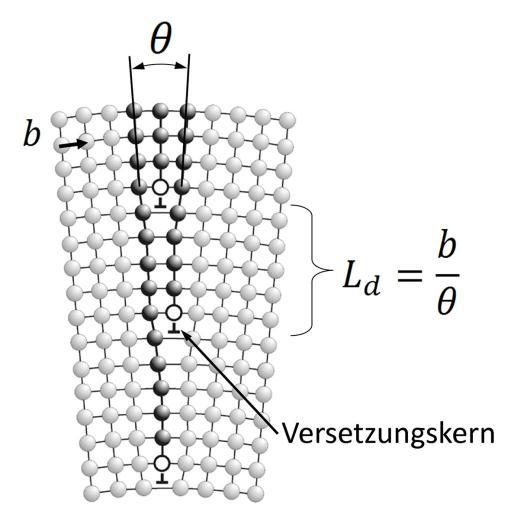
\includegraphics[scale=0.4]{Kleinwinkelkorngrenze.jpg}
\caption{Schematische Darstellung von Kleinkorngrenzen}
\end{figure}
\\\\
Bei genauerer Betrachtung erkennt man in obiger Abbildung eine Kette von aufeinander folgenden Stufenversetzungen. Zwischen zwei benachbarten Versetzungen erkennt man ein Dreieck. Der kleinste Winkel dieses Dreiecks ist der Versetzungswinkel \(\Theta\). Wenn dieser Winkel nicht zu groß ist, dann kann man das Dreieck in guter Näherung als rechtwinklig ansehen, wobei die beiden langen Seiten praktisch gleich groß sind. Ihre Länge ist etwa der Abstand \(L_{\mathrm{d}}\) der benachbarten Versetzungskerne. Die kurze Seite, die dem Winkel \(\Theta\) gegenüberliegt, ist für kleine Winkel etwa so groß wie die Gitterkonstante, d.h. so lang wie der Burgers-Vektor \(b=|\vec{b}|\). Dann gilt nach der Definition des Sinus am rechtwinkligen Dreieck:
\[\sin\Theta \approx \frac{b}{L_{\mathrm{d}}}\]
Da wir ohnehin nur die Kleinwinkelnäherung betrachten, kann man die Sinusfunktion auch noch linearisieren. Damit kann man den Versetzungswinkel leicht wie folgt abschätzen
\[\underline{\underline{\Theta \approx \frac{b}{L_{\mathrm{d}}}}}\]
Dies rechtfertigt nachträglich die Einteilung in Kleinwinkelkorngrenzen für Versetzungswinkel \(\Theta = 5^{\circ} \hdots 15^{\circ}\), denn das ist gerade der Winkelbereich, indem die Linearisierung der Sinusfunktion einen Fehler von nur wenigen Prozent bedeutet.

\subsection{Erster Versuchsteil: Silizium}
Versetzungen kann man durch Ätzverfahren sichtbar machen: Am Versetzungskern haben die Teilchen des Kristalls (Atome, Ionen,...) einen größeren Abstand zueinander und das Kristallgitter ist durch die Versetzung an dieser Stelle recht instabil. Dadurch können sich an dieser Stelle Teilchen leichter anlagern, sodass dort das Herauslösen in Folge des Ätzprozesses stattfinden kann. Die Strategie besteht also darin, den Kristall zuerst möglichst glatt zu schleifen und chemisch zu polieren um eine sehr ebene Oberfläche zu erzeugen und diese anschließend zu ätzen. An den Stellen mit Stufenversetzungen bilden sich dann in der ansonsten glatten Oberfläche deutlich sichtbare Ätzgrübchen. Aus diesen lassen sich dann wertvolle Informationen über den Kristall gewinnen:
\begin{itemize}
\item Die Ätzgrübchen bilden je nach Orientierung der Kristallebene sehr charakteristische Formen aus. Die Orientierung des Kristalls lässt sich somit ohne Beugungsverfahren mit Röntgenstrahlung bestimmen.
\item Bei einer Häufung vieler Ätzgrübchen kann man die Anzahl der Ätzgrübchen pro Fläche zählen. Aus dieser lässt sich dann eine Versetzungsdichte berechnen. Diese ist ein Maß für die Abweichung von der Idealstruktur.
\item Erkennt man eine Linie von Ätzgrübchen ist das ein Hinweis auf eine sogenannte Subkorngrenze. Dort besteht ein Versetzungswinkel zwischen verschiedenen Bereichen des Kristalls.  Durch Ausmessen des Abstandes benachbarter Ätzgrübchen kann bei Kenntnis der Gitterkonstanten dieser Versetzungswinkel \(\Theta\) abgeschätzt werden. Auch dieser ist ein Maß dafür, wie stark die Kristallstruktur vom Idealfall abweicht.
\end{itemize}
Im Fall von Silizium erhält man folgende charakteristischen Formen in Abhängigkeit von der Orientierung:
\begin{enumerate}
\item quadratische Ätzgrübchen für die \(\left\lbrace 100 \right\rbrace\) Richtung.
\item linsenförmige Ätzgrübchen für die \(\left\lbrace 110 \right\rbrace\) Richtung.
\item Ätzgrübchen in Form gleichseitiger Dreiecke für die \(\left\lbrace 111 \right\rbrace\) Richtung.
\end{enumerate}
wobei andere Richtungen wie etwa \(\left\lbrace 215 \right\rbrace\) im Allgemeinen keine leicht oder gar eindeutig zu identifizierenden Ätzgrübchen hervorbringen. Die Herkunft dieser charakteristischen Formen ist in nachfolgender Abbildung dargestellt:
\begin{figure}[h!]\centering
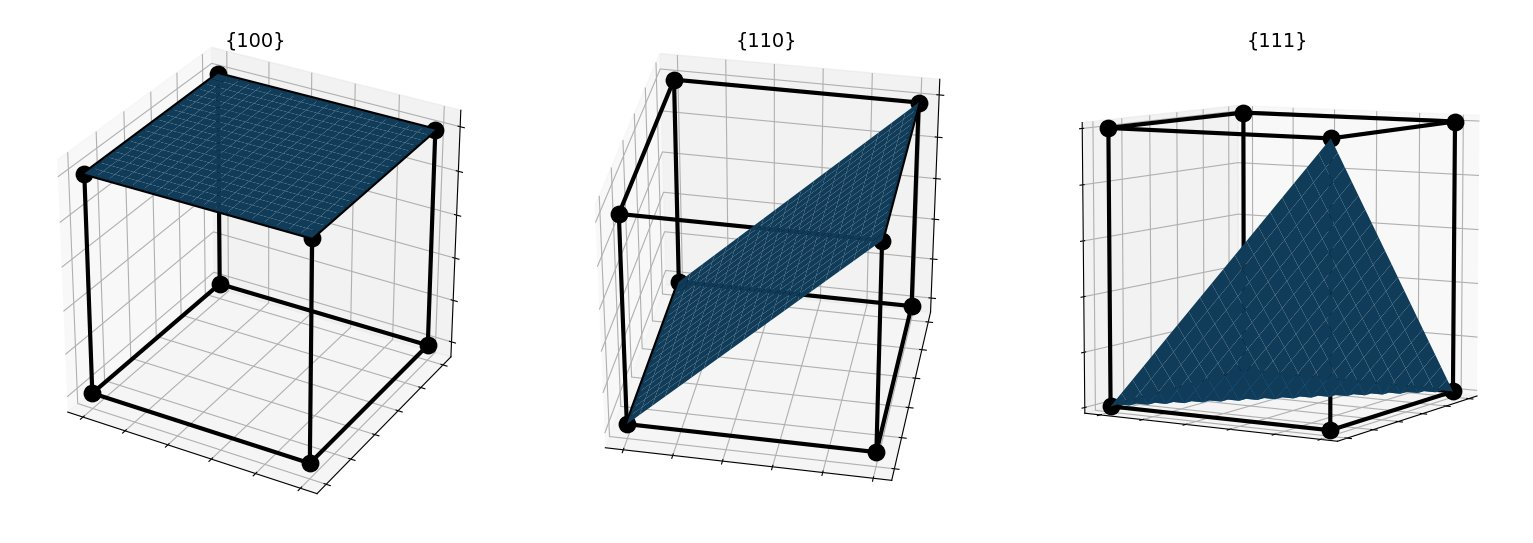
\includegraphics[width=\textwidth]{Aetzgruebchen_Modell.jpg}
\caption{Modell zur Erklärung der Form der Ätzgrübchen in Abhängigkeit von den \textsc{Miller}schen Indices der Kristallebene}
\end{figure}



\subsection{Zweiter Versuchsteil: Stahl und Messing}
\subsubsection{Stahl}
Stahl ist eine Eisen-Kohlenstoff-Legierung. Bis zu einem Kohlenstoffanteil von 2,06 \% werden solche Legierungen als Stahl bezeichnet. Der Anteil an Kohlenstoff bestimmt dabei wesentlich, ob der entstehende Stahl gehärtet werden kann sowie die Zugfestigkeit und Streckgrenze. Ab 2,06 \% Kohlenstoffanteil ist die Legierung nicht mehr schmiedbar und muss gegossen werden, deshalb wird sie dann als Gusseisen bezeichnet. Eisen-Kohlenstoff-Legierungen mit mehr als 6,67 \% Kohlenstoffanteil bilden Eisencarbid \(\mathrm{Fe}_3\mathrm{C}\), dass man auch Zementit nennt. Solche Verbindungen sind zu spröde um sie technisch nutzbar zu machen; sie dienen lediglich als Ausgangspunkt für andere Legierungen. Der Kohlenstoffanteil bestimmt also maßgeblich die Eigenschaften des Materials. \\\\
Wird die Oberfläche des Stahls angeätzt, kann man die verschiedenen Mischkristalle im Material erkennen. Perlit (Gemenge aus Zementit und Ferrit) bildet dabei dunkle Bereiche; das reine Eisen (Ferrit) dagegen helle Bereiche. Durch Bestimmung der Flächenanteile kann man dann zunächst den Volumenanteil an Perlit ermitteln und aus dessen Dichte den zugehörigen Massenanteil. Da die Atommassen von Eisen und Kohlenstoff sowie die Summenformel von Zementit (\(\mathrm{Fe}_3\mathrm{C}\)) bekannt sind, lässt sich der Massenanteil von Kohlenstoff im Stahl errechnen.



\subsubsection{Messing}
Messing ist eine Legierung aus Kupfer und Zink. Je nach Zinkgehalt unterscheidet man zwischen $\alpha$-, $\beta$- und $\gamma$-Messing. Für diesen Versuch sind  $\alpha$- und $\beta$-Messing von Bedeutung. Diese haben einen Zinkgehalt von über $62,5$\% für die \(\alpha\)-Phase bzw. $45$\%-$50$\% für die \(\beta\)-Phase. Die beiden Phasen bilden unterschiedliche Kristallstrukturen: $\alpha$- Messing ordnet sich in einem kubisch-flächenzentrierten (kfz) und $\beta$- Messing in einem kubisch-raumzentrierten (krz) Gitter an. Im durchzuführenden Ätzen des Messings werden die $\beta$- Mischkristalle aufgrund des geringeren Kupfer- und höheren Zinkanteils zuerst angegriffen. Nach dem Ätzvorgang erscheinen diese stärker angegriffenen Bereiche der Metalloberfläche als dunklere Stellen. Auf diese Weise kann man die verschiedenen Phasen erkennen und deren Volumenanteil durch stereologische Methoden ermitteln. Unter Berücksichtigung der Dichten der verschiedenen Phasen kann der Massenanteil jedes Mischkristalls dann errechnet werden. Da zudem von \(\alpha\)- und \(\beta\)-Messing jeweils der Zinkgehalt bekannt ist, kann schließlich auf den Zinkanteil der gesamten Probe geschlossen werden.


\section{Durchführung}
\subsection{Erster Teilversuch: Silizium}
\begin{itemize}
\item Läppen: Reiben des gegebenen Siliziumkörpers auf einer Glasplatte mit Läpppulver F40 und Wasser für einige Minuten zur Glättung der Oberfläche
\item 1. Ätzschritt: 25s in einer Mischung aus $10$ ml Flusssäure und $10$ ml Salpetersäure zum chemischen Abtragen der Oberfläche
\item Betrachten unter dem Mikroskop und Aufnahme von Bildern
\item 2. Ätzschritt: 30s in einer Mischung aus $5$ ml Flusssäure und $25$ ml Salpetersäure zum chemischen Polieren der Oberfläche
\item erneute Betrachtung unter dem Mikroskop und Aufnahme von Bildern
\item 3. Ätzschritt: 15s in einer Mischung aus $10$ ml Stammlösung (50g \(\mathrm{CrO}_3\) auf 100ml \(\mathrm{H}_2\mathrm{O}\)) und $10$ ml Flusssäure zur deutlichen Herausbildung von Ätzgrübchen.
\item Betrachtung unter dem Mikroskop und Aufnahme von Bildern, Hauptuntersuchung der nun freigelegten Strukturen
\end{itemize}
Der Kristall wurde nach jedem Ätzschritt zuerst mit reichlich destilliertem Wasser gespült und danach für drei Minuten in Ethanol im Ultraschallbad gereinigt um jegliche Reste der Säure zu entfernen. Um die Dimensionen der aufgelösten Strukturen einschätzen zu können, wurde den Bildern nachträglich ein Maßstab hinzugefügt. Es ergaben sich folgende Aufnahmen: \\\\
\begin{minipage}{0.45\textwidth}\centering
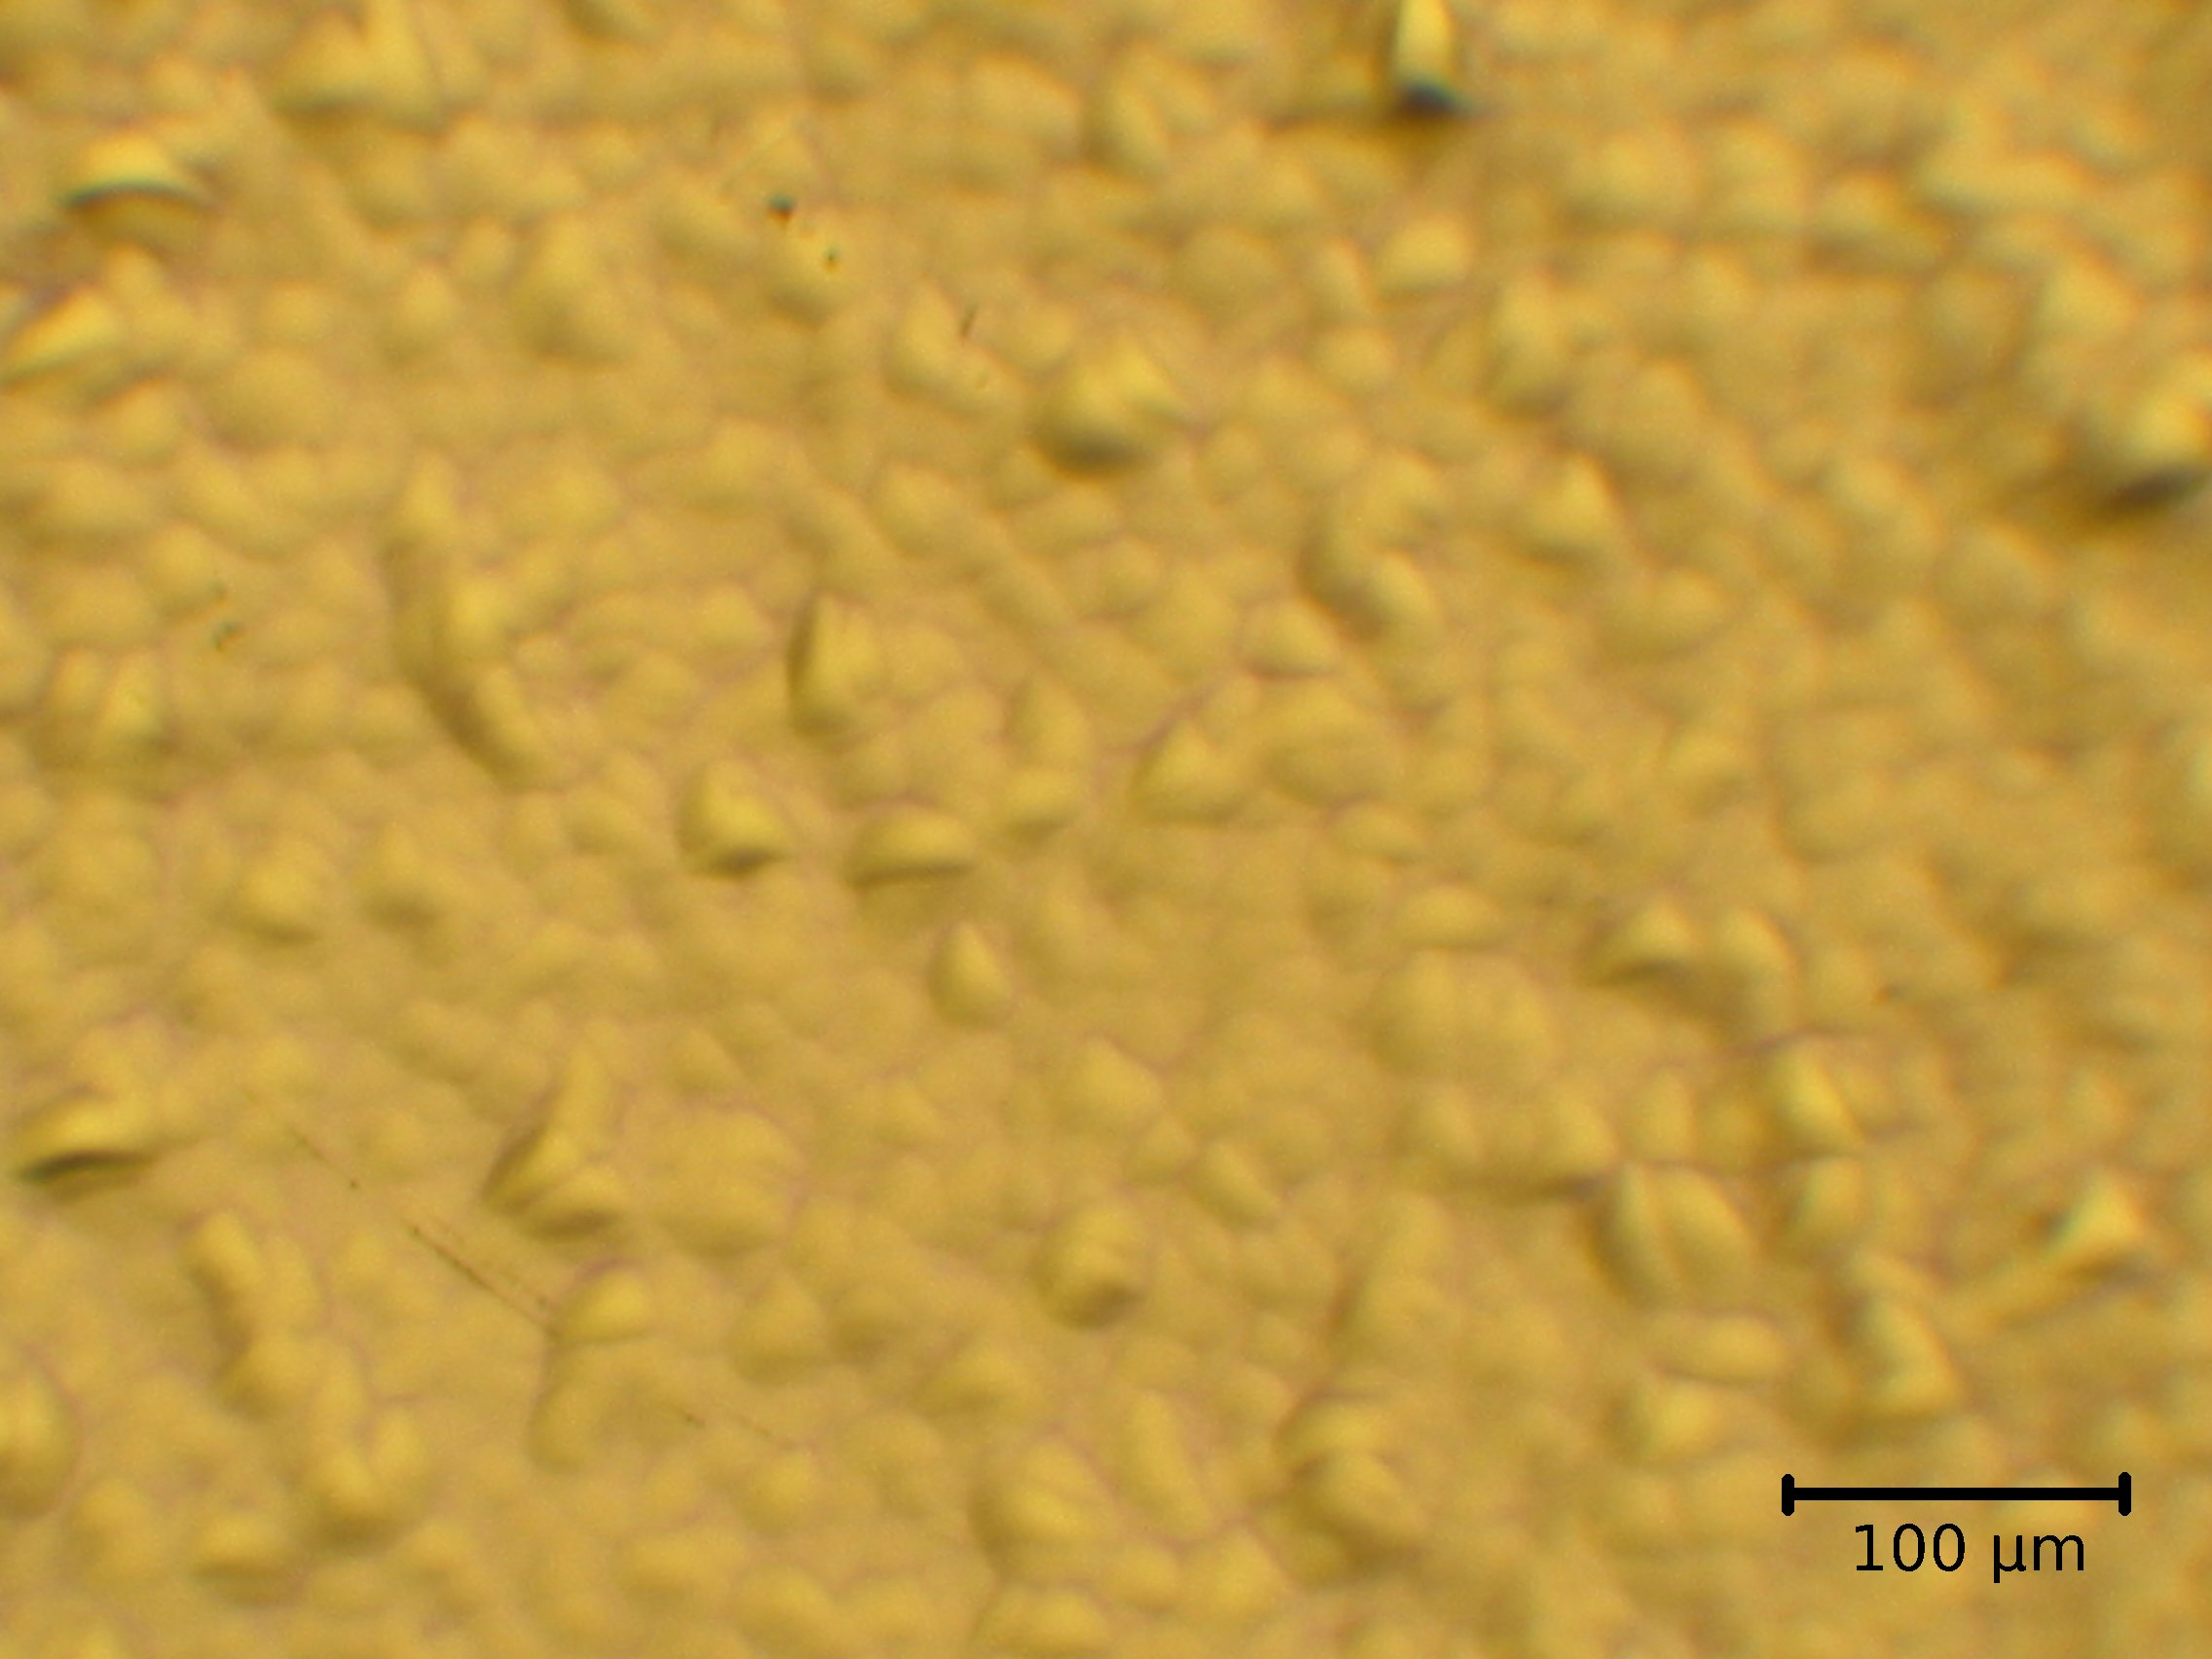
\includegraphics[scale=0.09]{Si_1Sch_25s_12_5x_00002.jpg}
\captionof{figure}{Silizium, 1.Ätzung, 12.5fach}
\end{minipage}
\begin{minipage}{0.1\textwidth}\centering
\[\]
\end{minipage}
\begin{minipage}{0.45\textwidth}\centering
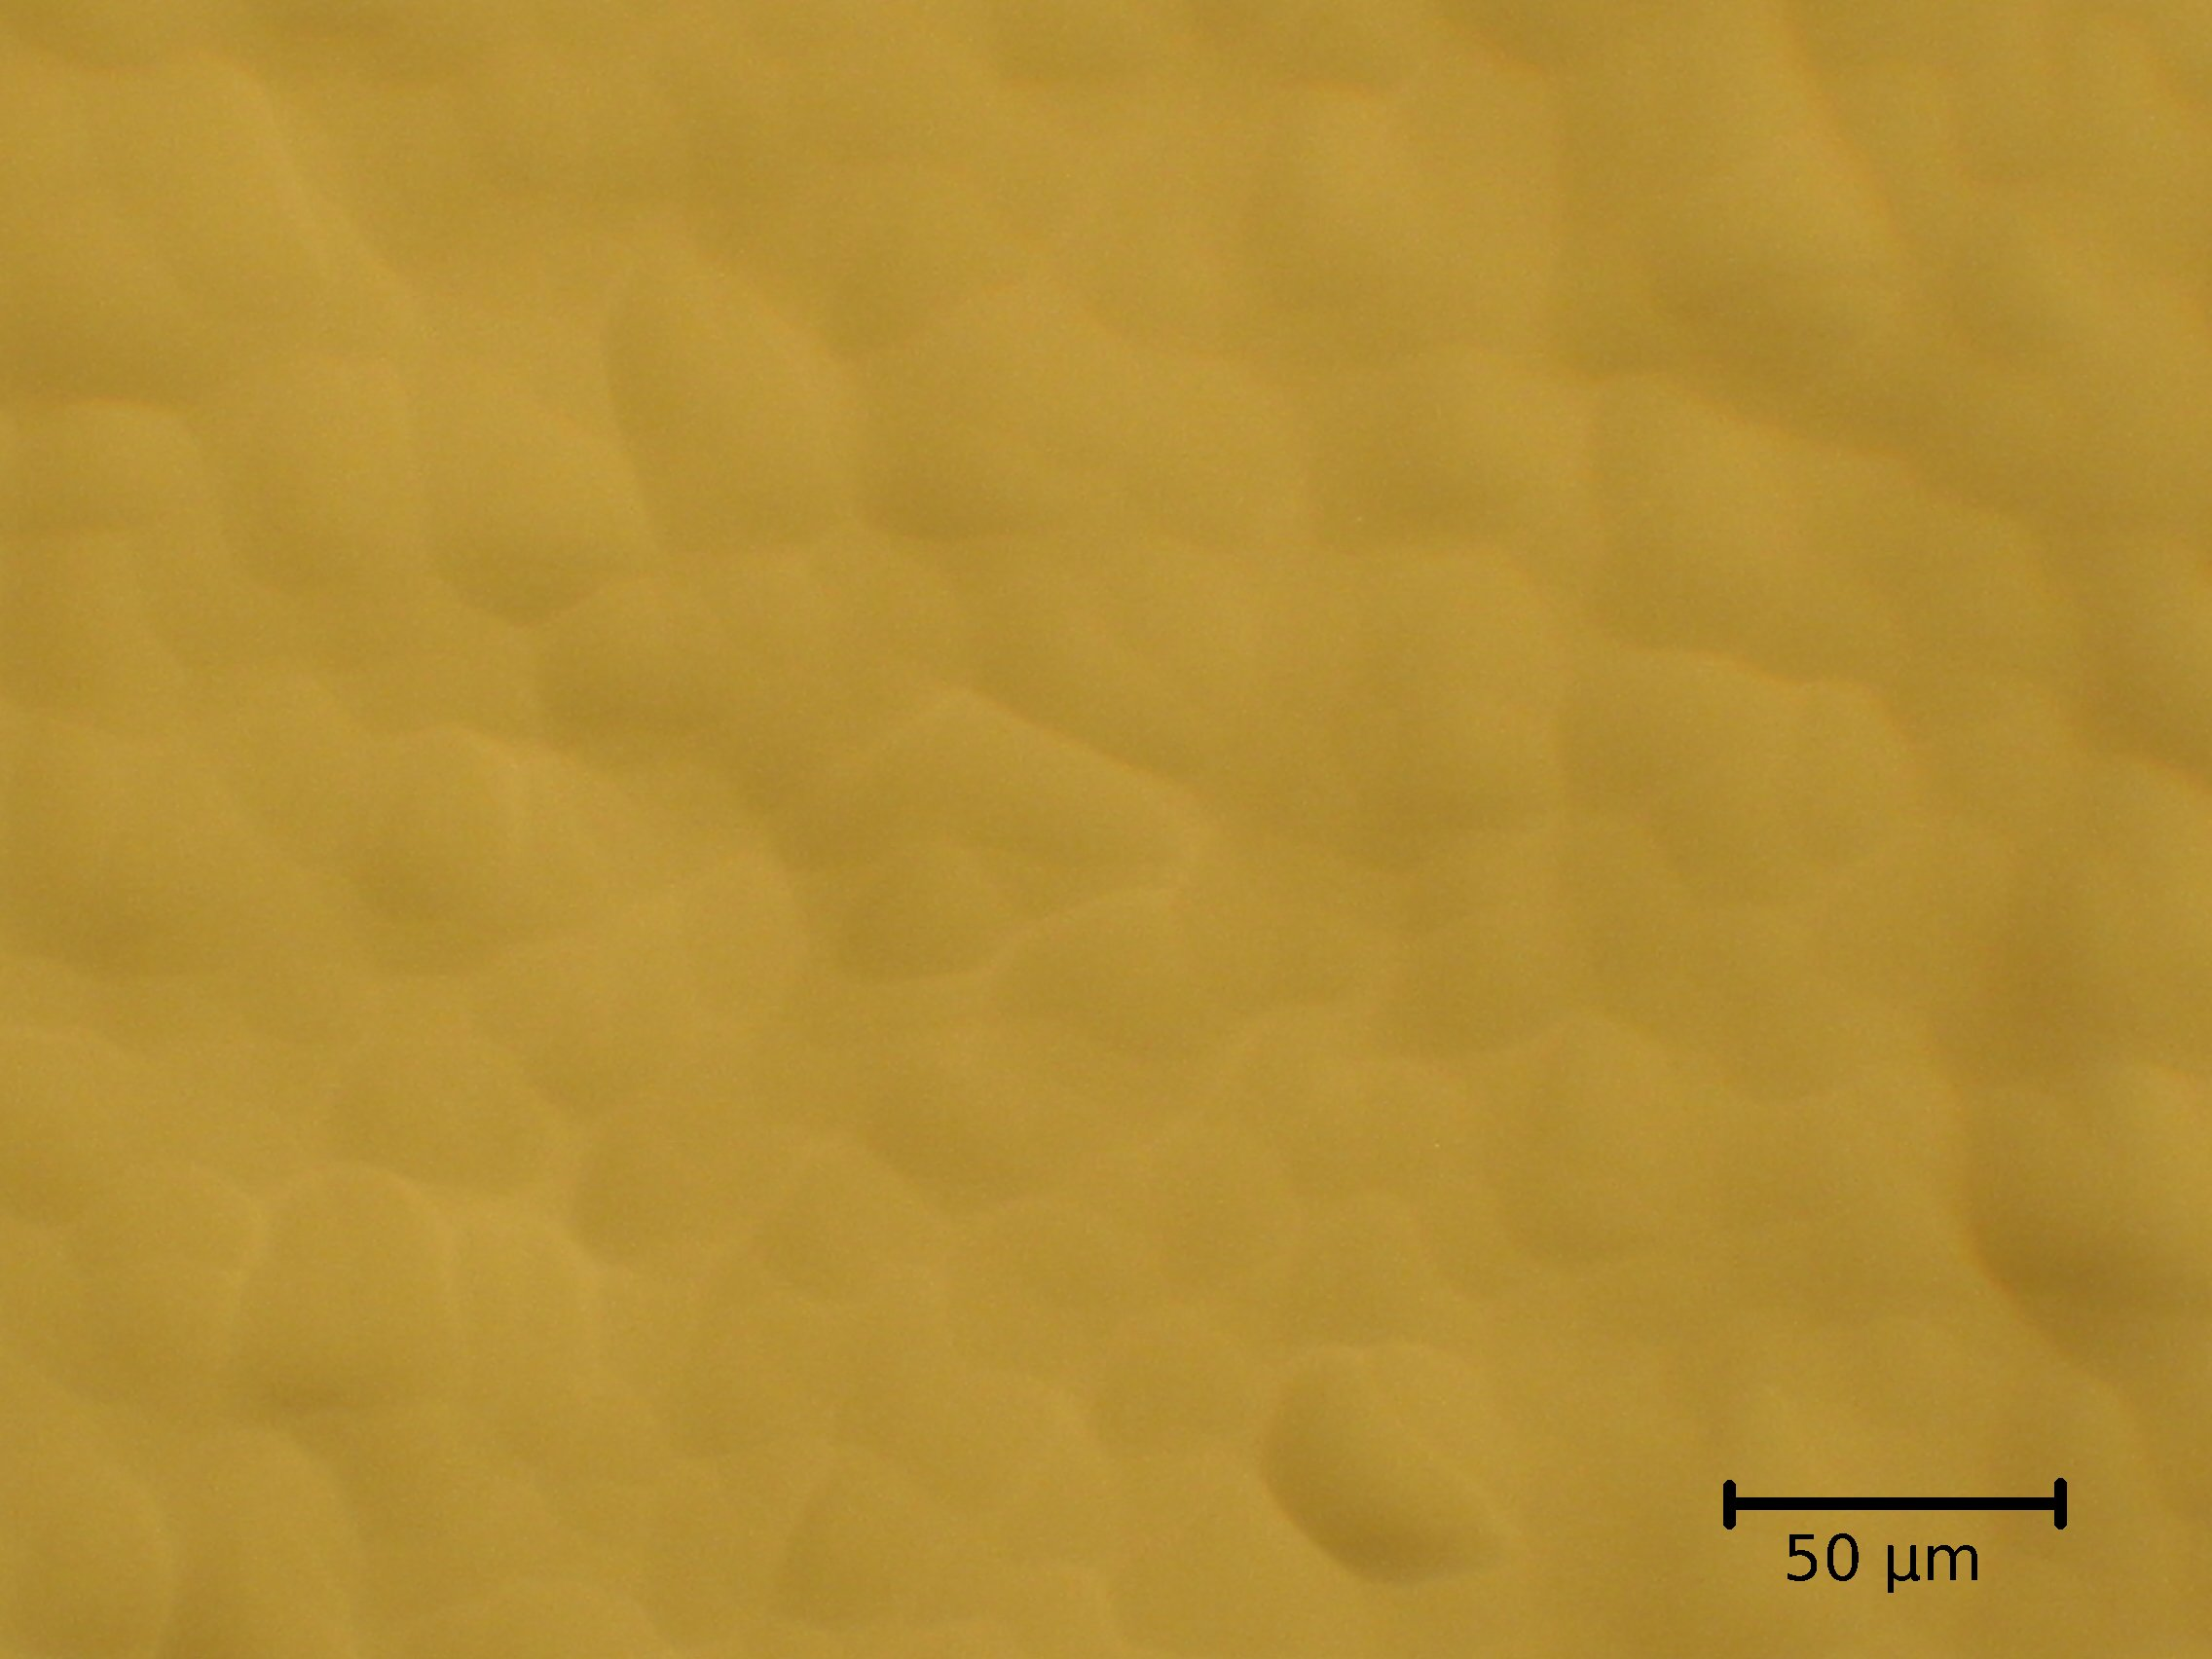
\includegraphics[scale=0.09]{Si_1Sch_25s_25x_00006}
\captionof{figure}{Silizium, 1.Ätzung, 25fach}
\end{minipage} \\


\begin{minipage}{0.45\textwidth}\centering
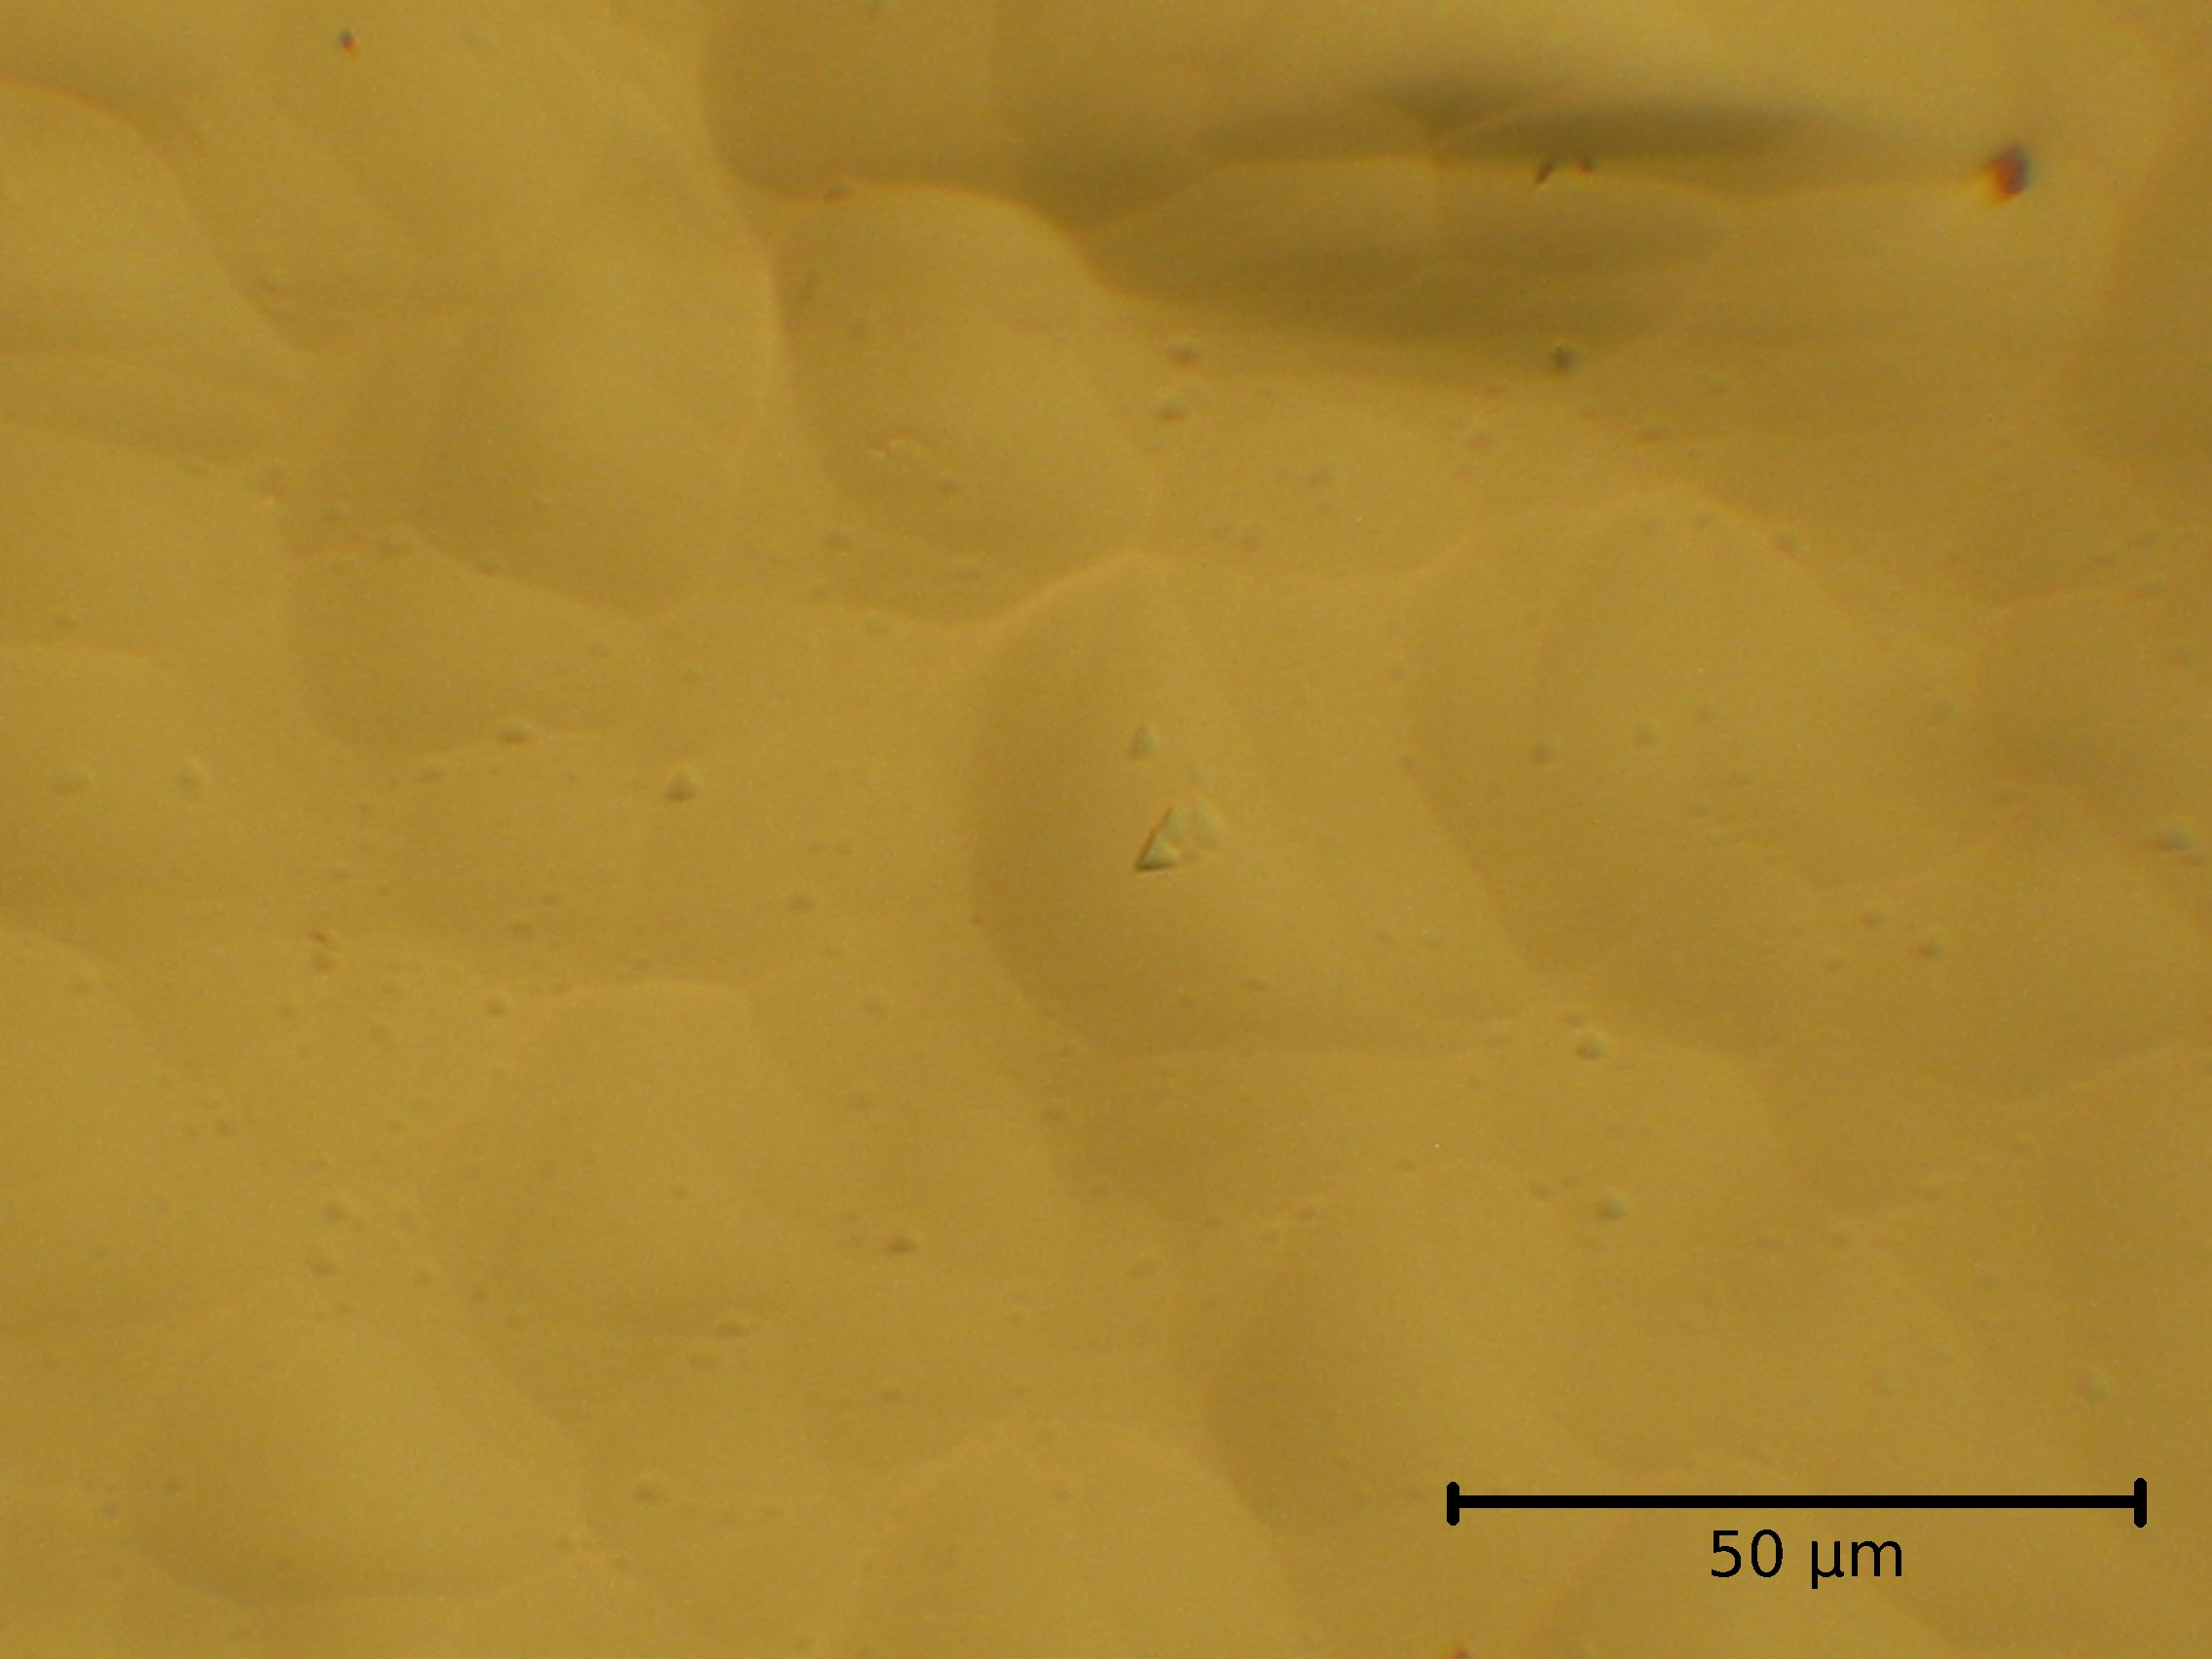
\includegraphics[scale=0.09]{Si_2Sch_30s_2x25x_00010}
\captionof{figure}{Silizium, 2.Ätzung, 50fach}
\end{minipage} \\\\


\begin{minipage}{0.45\textwidth}\centering
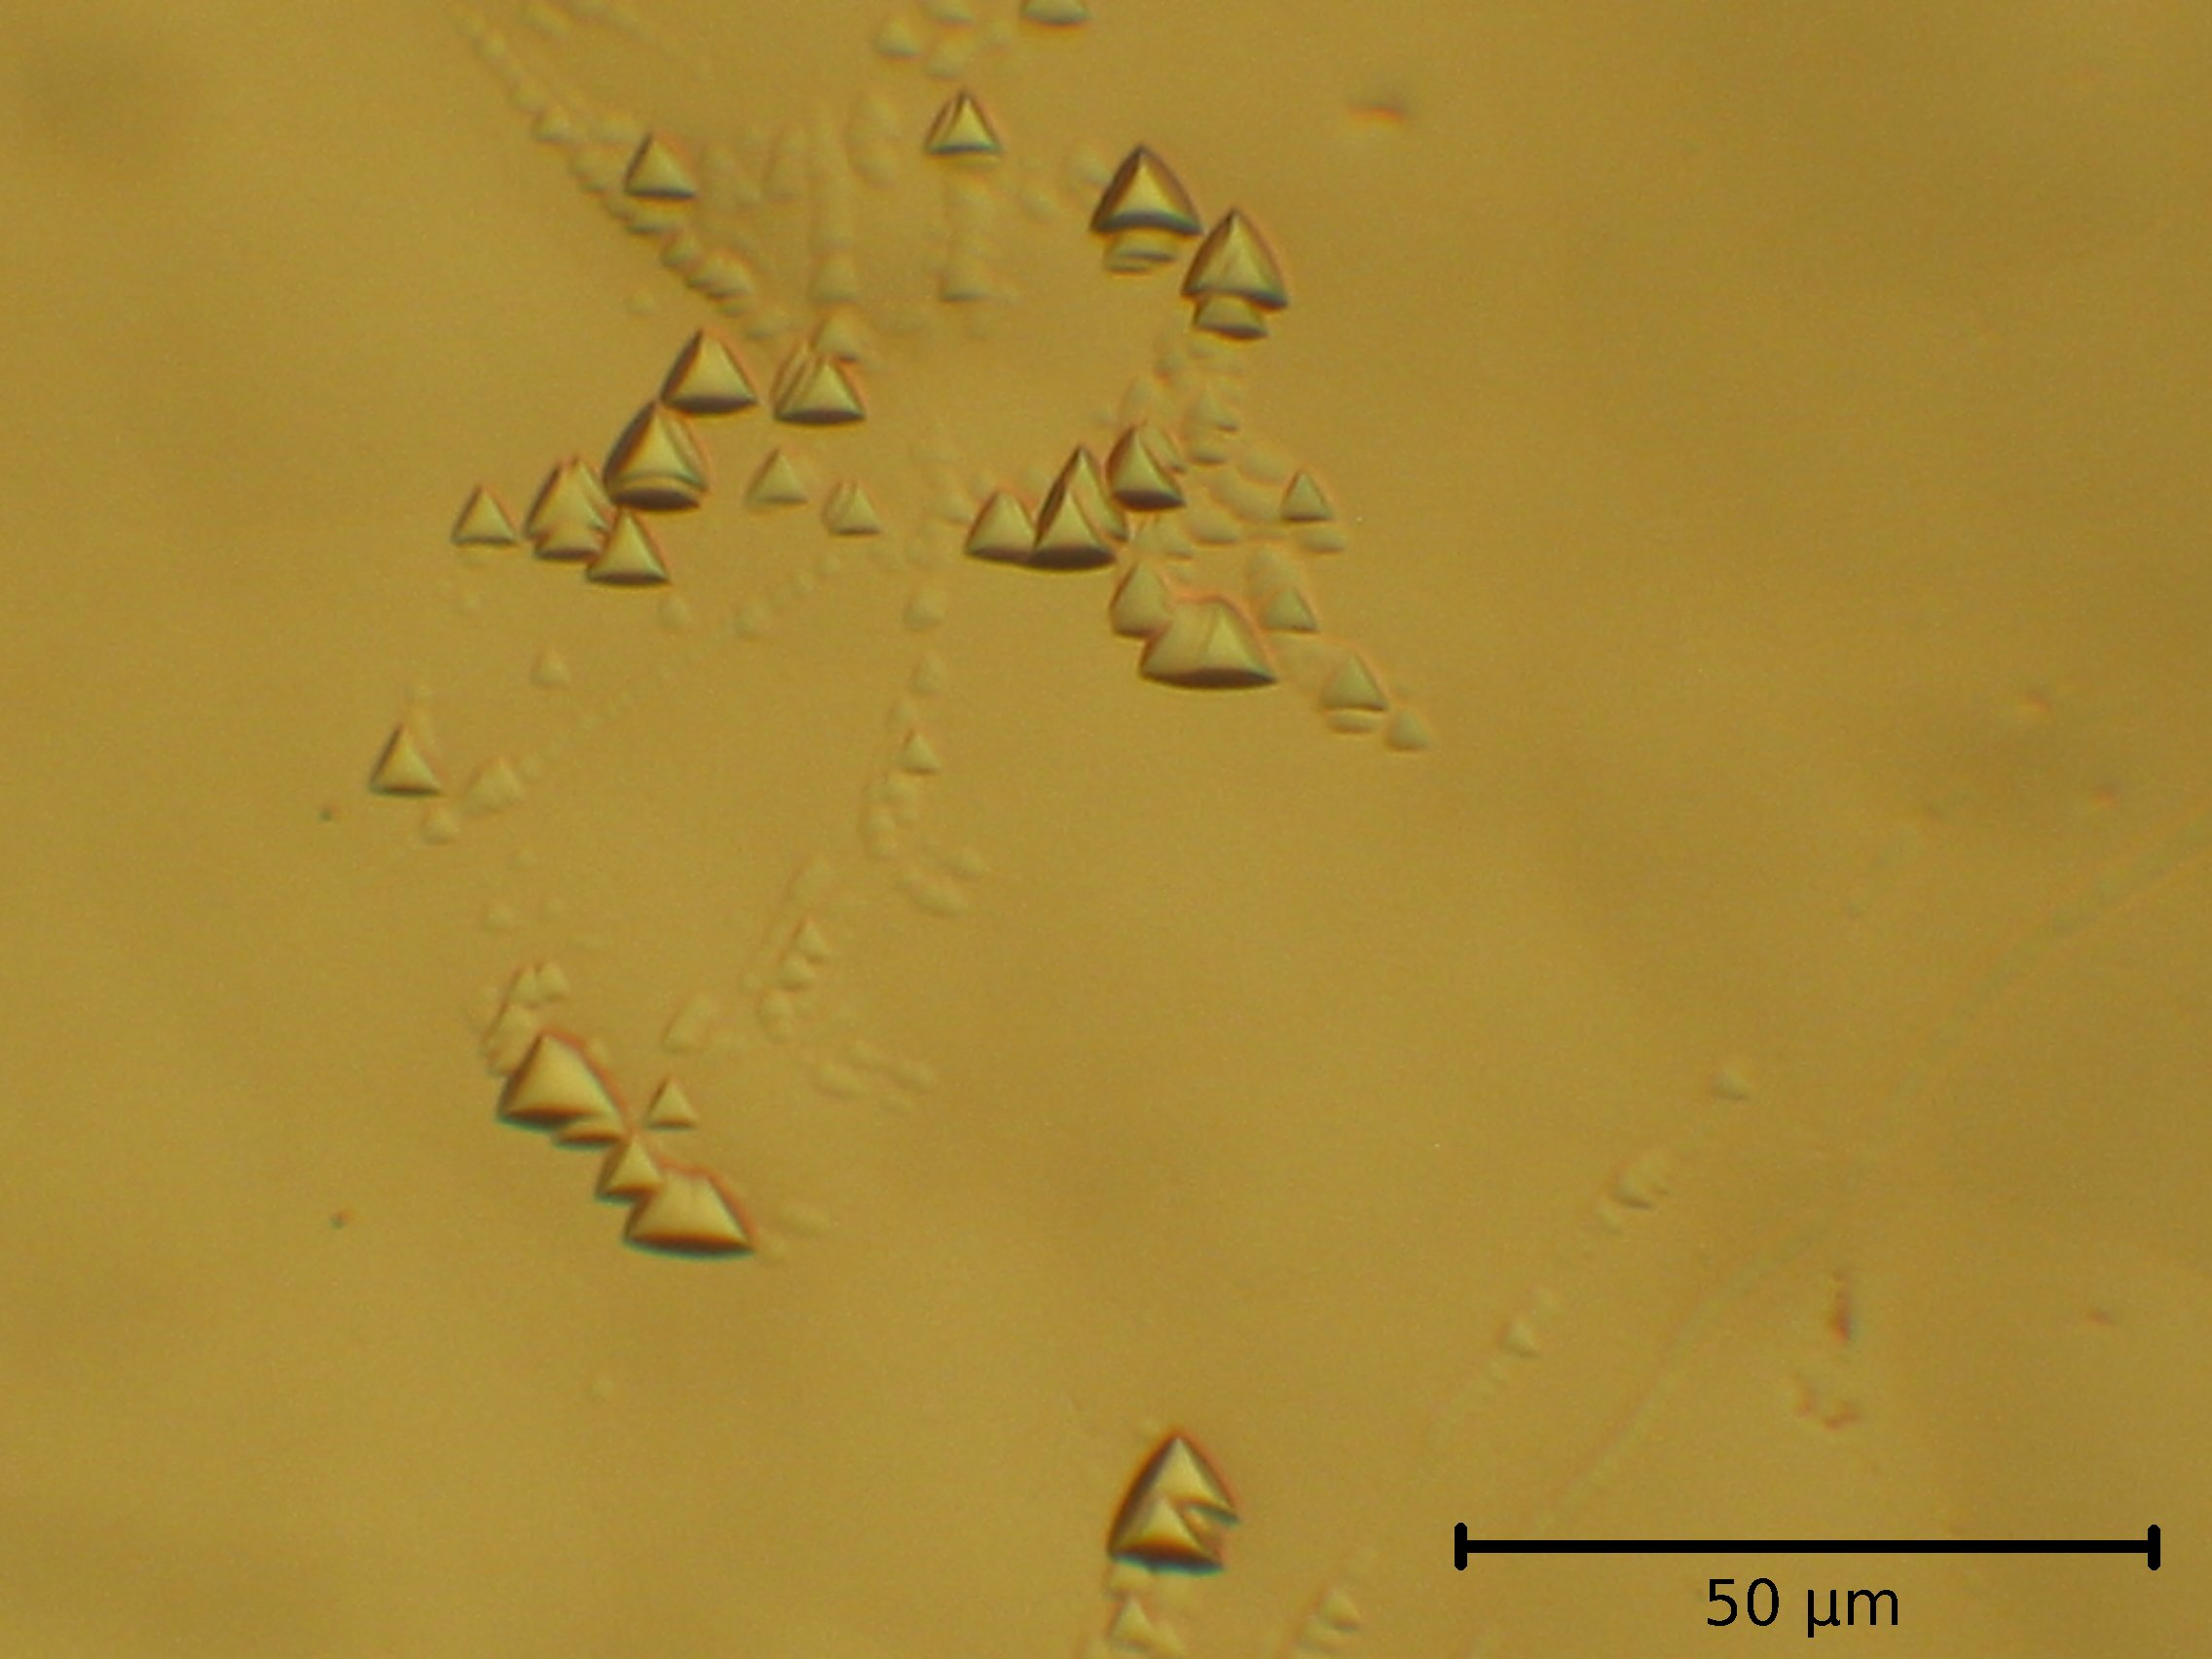
\includegraphics[scale=0.08]{Si_3Sch_15s_2x25x_00018}
\captionof{figure}{Silizium, 3.Ätzung, 50fach}
\end{minipage}
\begin{minipage}{0.1\textwidth}\centering
\[\]
\end{minipage}
\begin{minipage}{0.45\textwidth}\centering
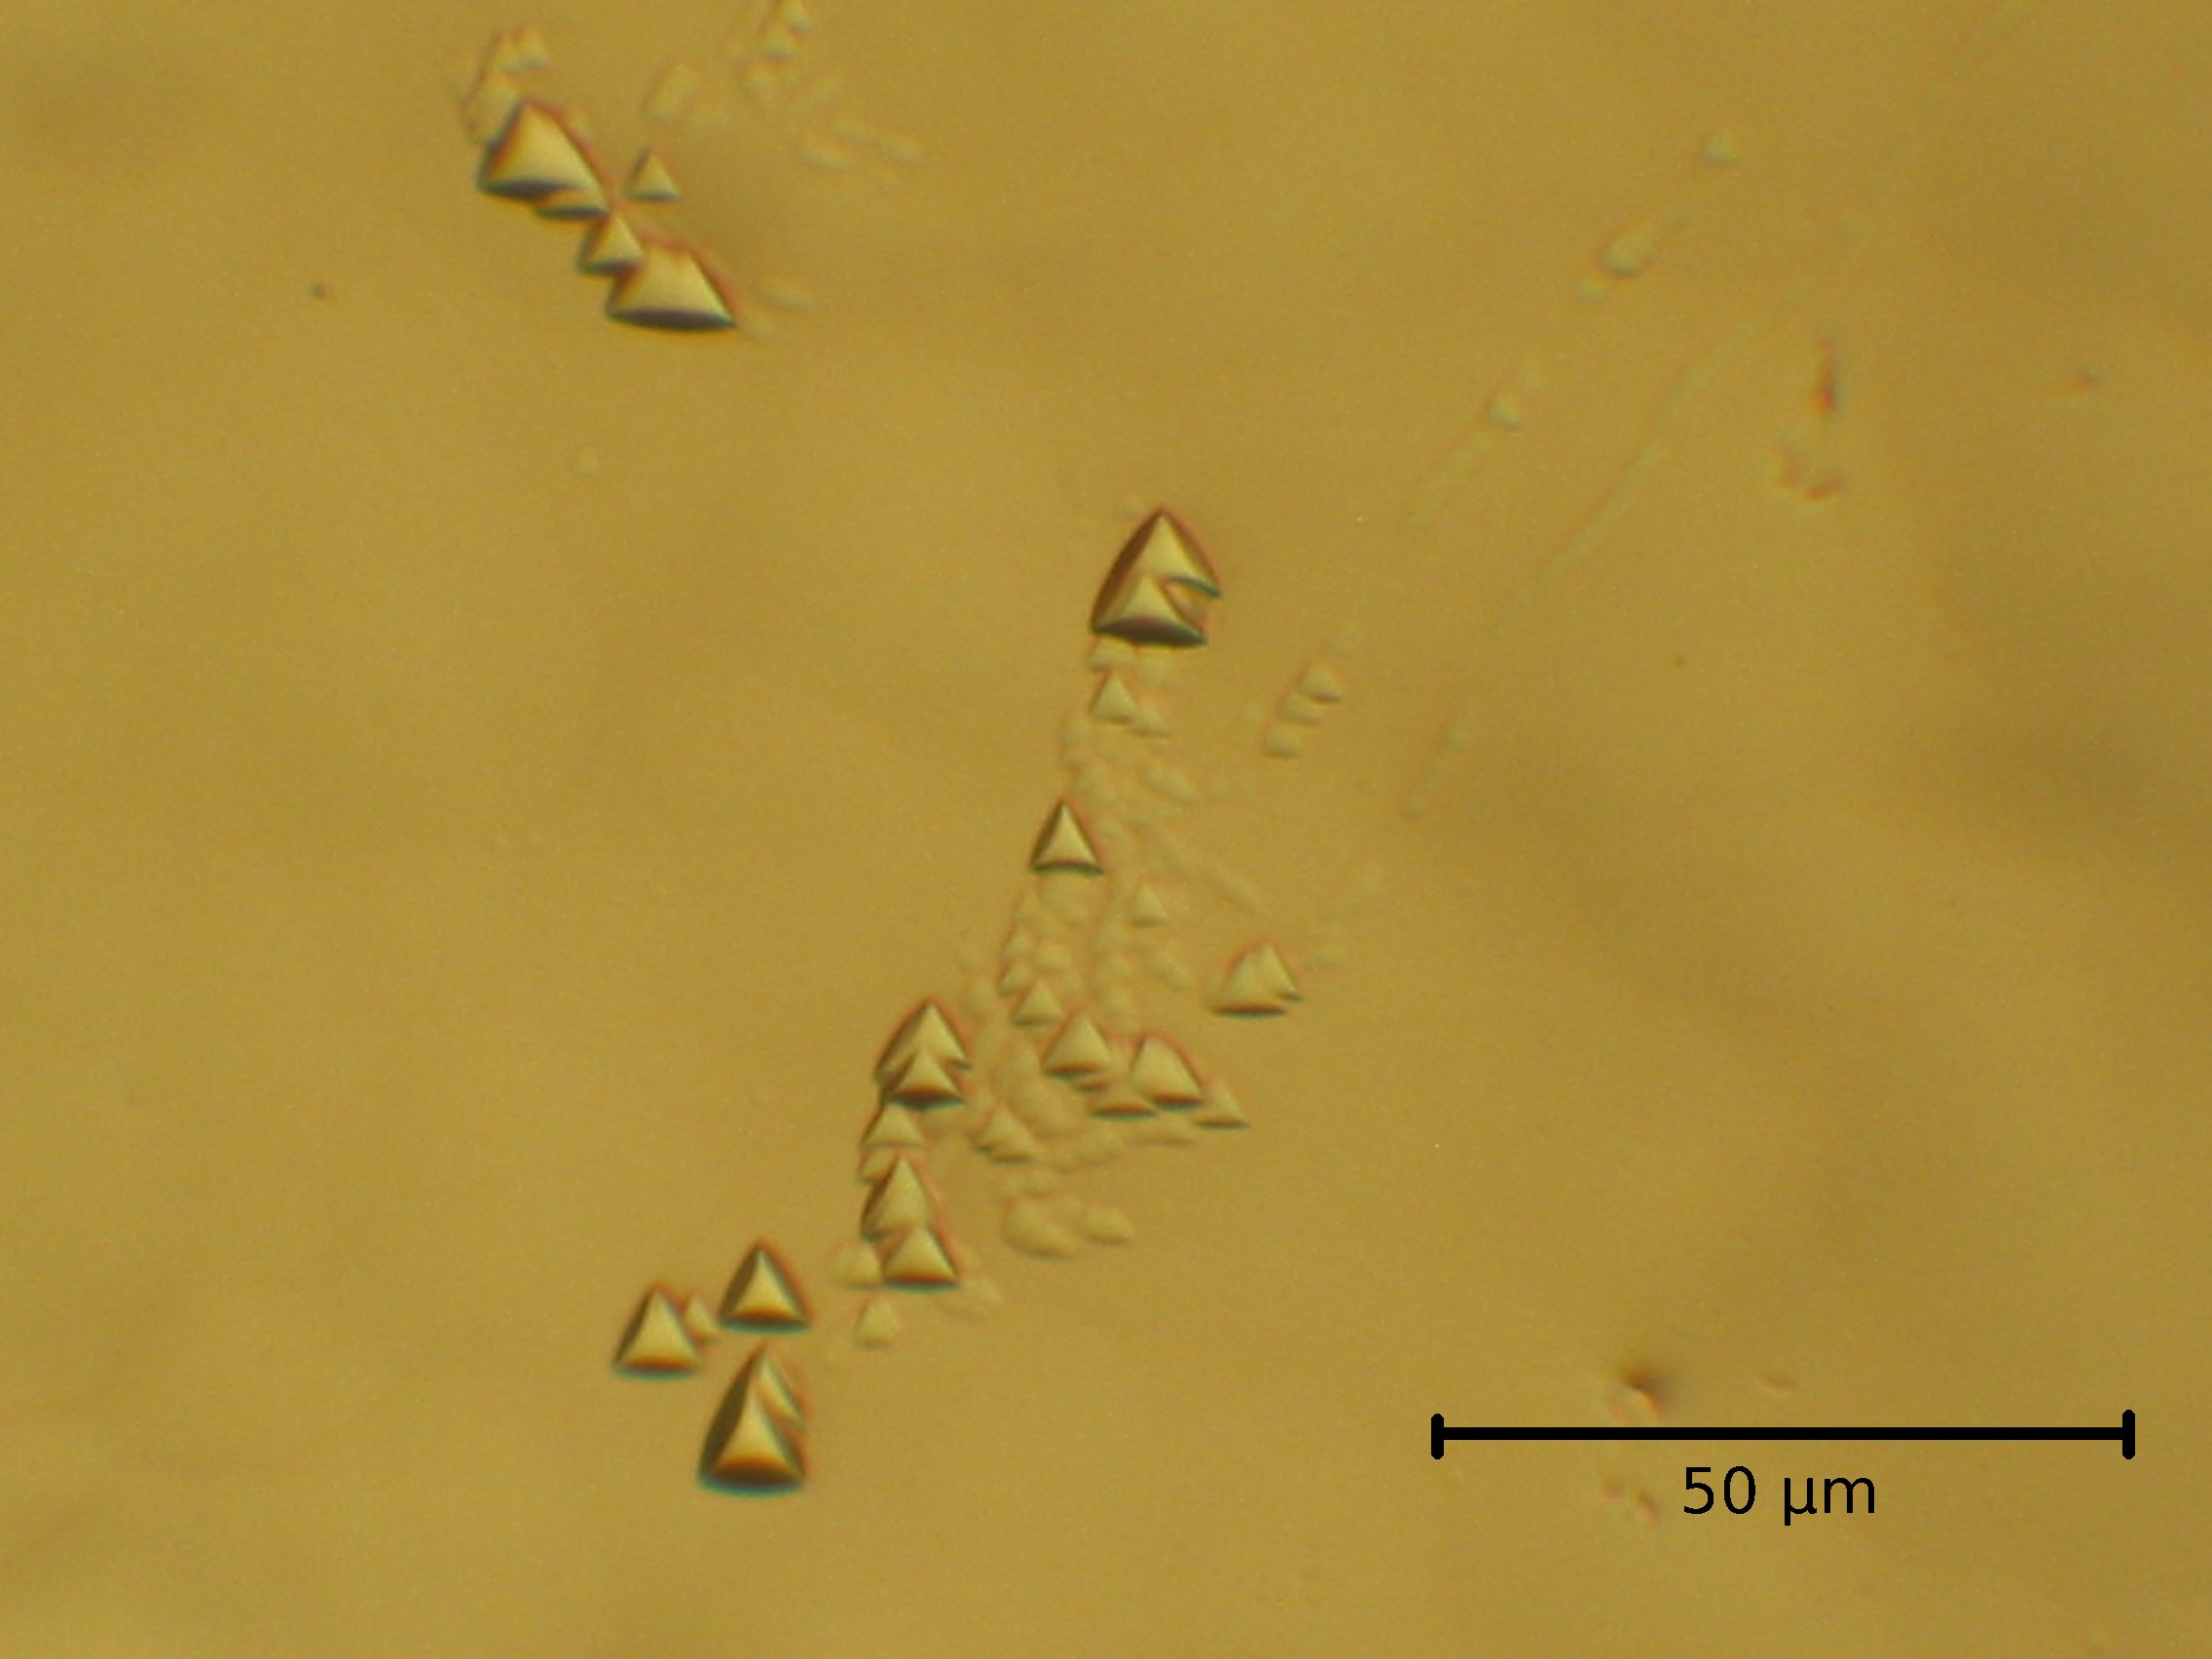
\includegraphics[scale=0.08]{Si_3Sch_15s_2x25x_00019}
\captionof{figure}{Silizium, 3.Ätzung, 50fach}
\end{minipage} \\\\
\begin{minipage}{0.45\textwidth}\centering
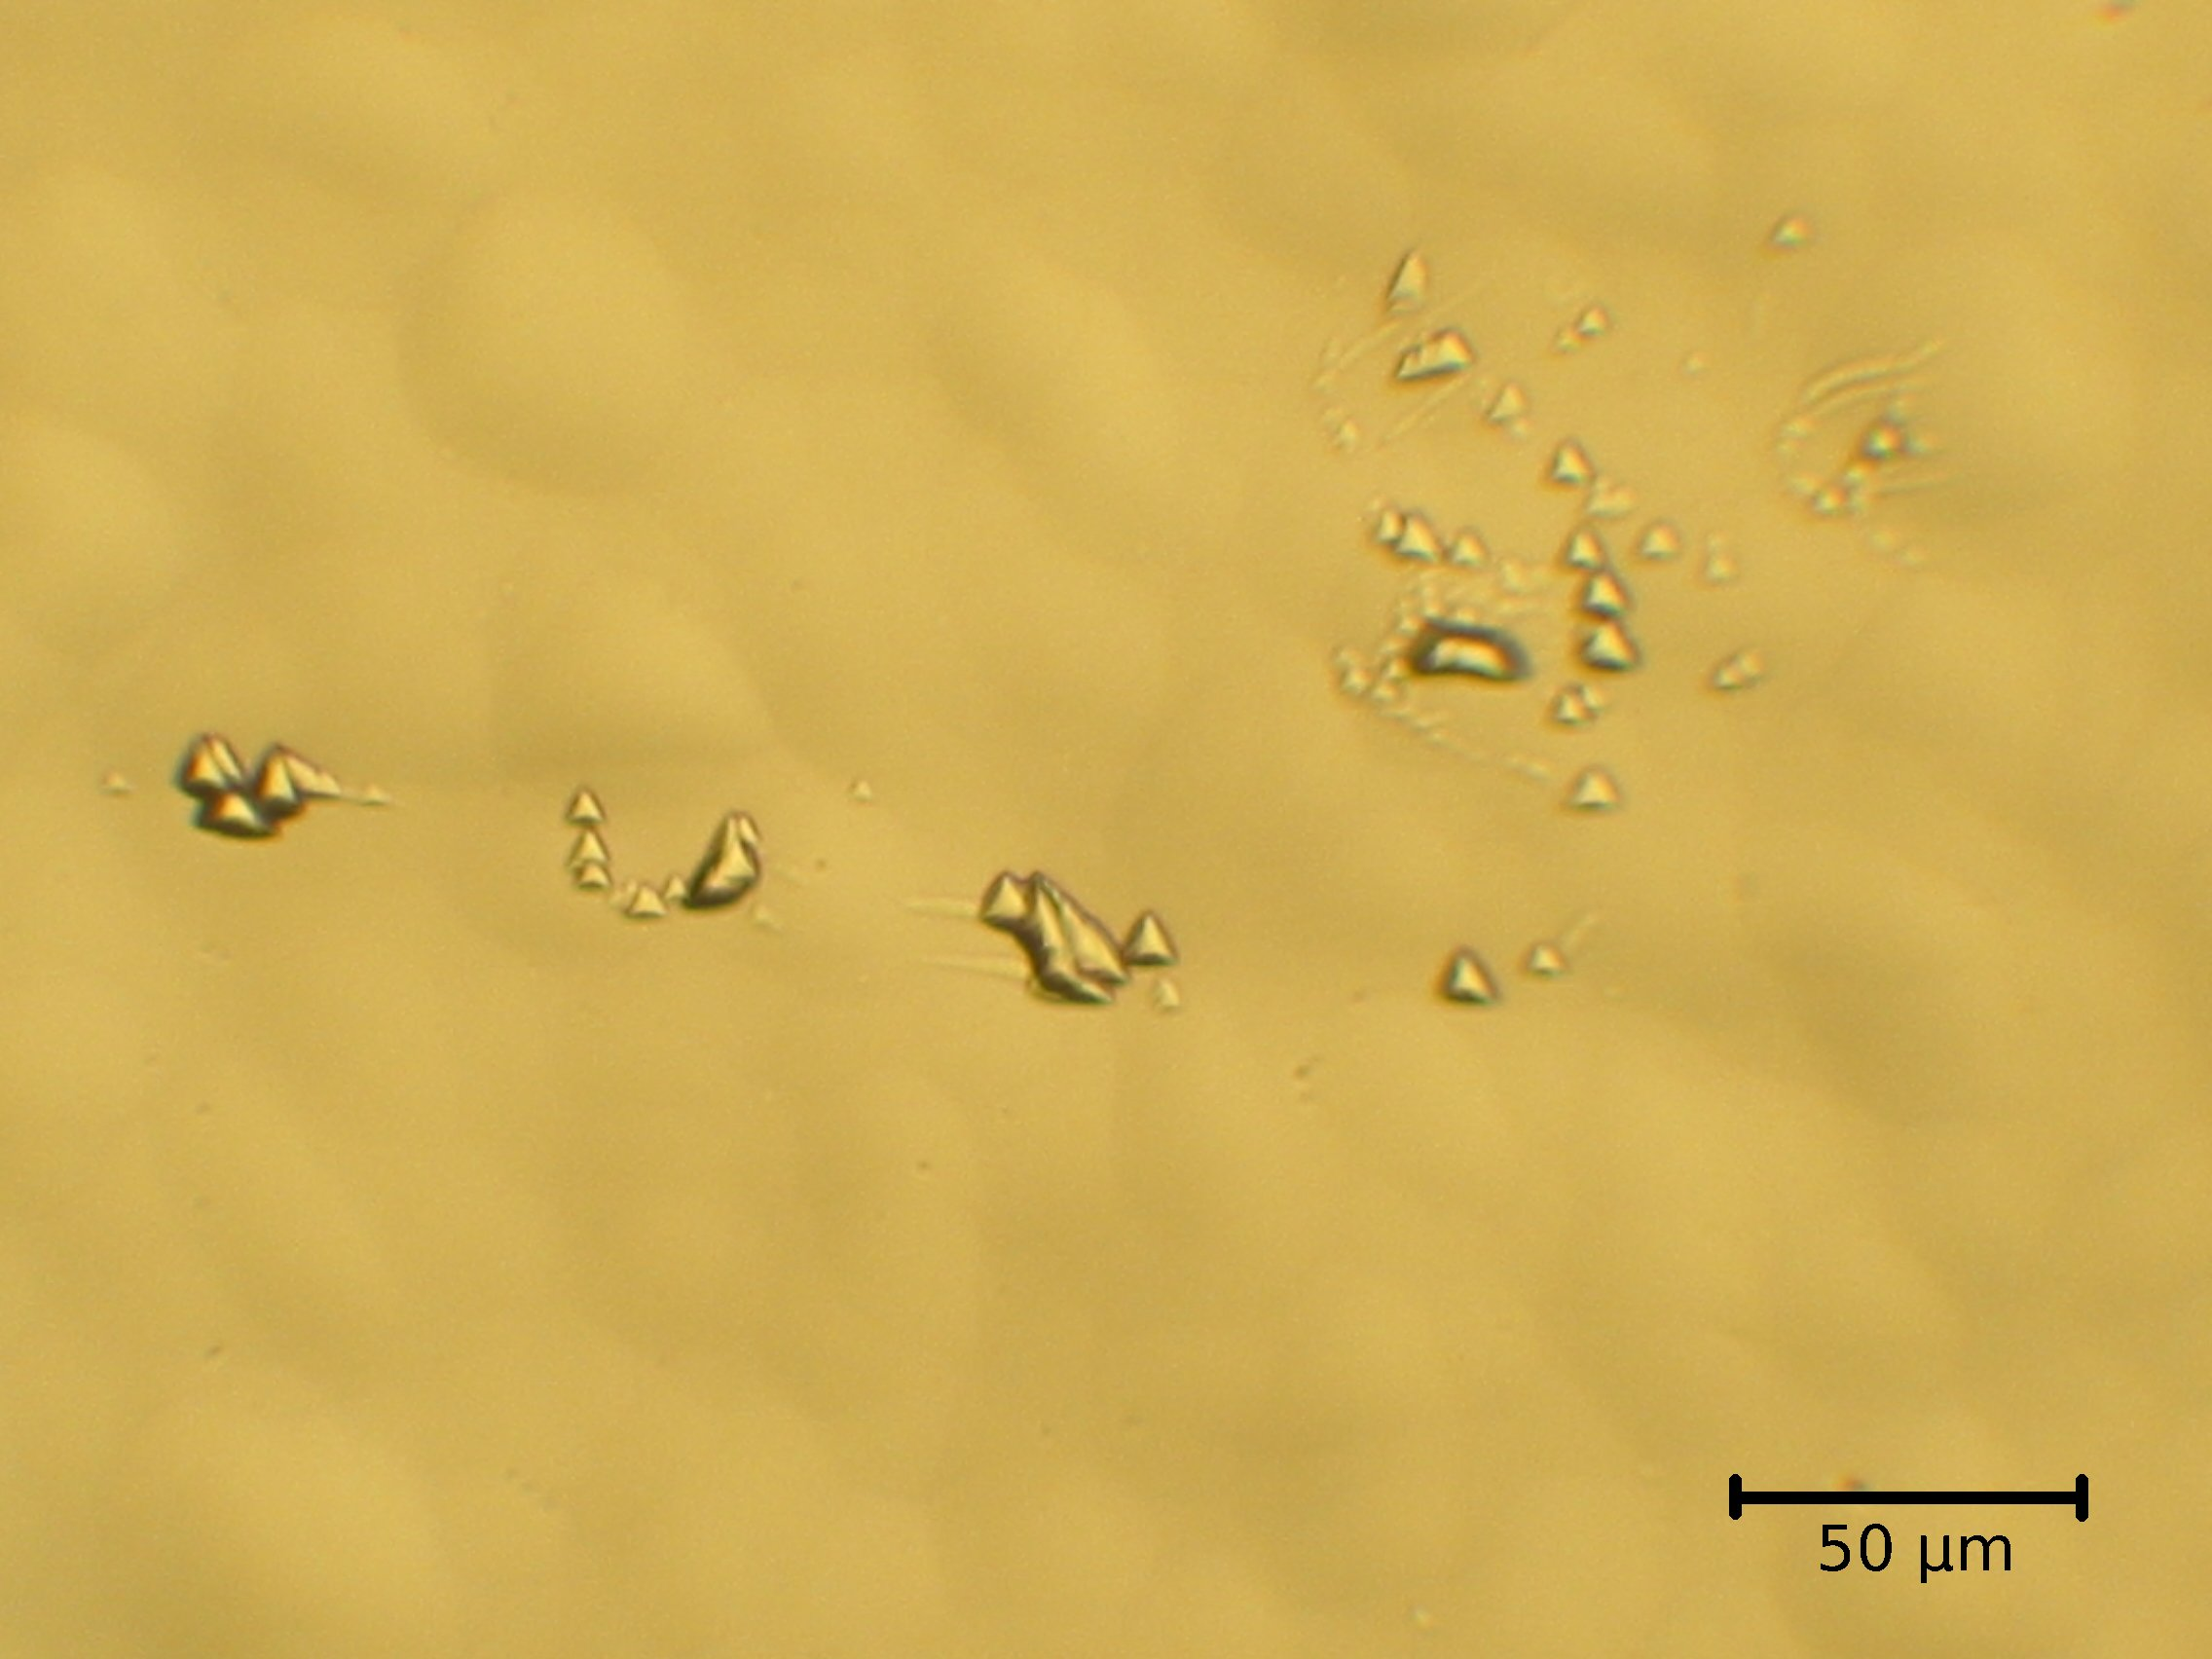
\includegraphics[scale=0.08]{Si_3Sch_15s_25x_00017}
\captionof{figure}{Silizium, 3.Ätzung, 25fach}
\end{minipage}
\\\\\\
Bei den Abbildungen 9 bis 11 ist nun also deutlich die dreieckige Form der Ätzgrübchen zu erkennen.

\subsection{Zweiter Teilversuch: Stahl und Messing}
Für die Probekörper (Zylinder) aus Messing und Stahl wurden vorerst dieselben Arbeitsschritte angewendet:
\begin{itemize}
\item Nassschleifen der Körper mit SiC-Schleifpapier der Körnungen 500, 1000 und 2400 (in dieser Reihenfolge)
\item Polieren mit 3\(\mu\)m Diamantsuspension, bis die Oberfläche metallisch glänzt
\end{itemize}
Anschließend erfolgte das Ätzen, wobei ab jetzt Messing und Stahl verschieden behandelt wurden:
\begin{itemize}
\item Ätzen des Stahls für 5s in 3\%-iger alkoholischer Salpetersäure
\item Ätzen des Messings für 25s in einer Mischung aus 100ml \(\mathrm{H}_2\mathrm{O}\), 30ml \(\mathrm{HCl}\) und 5g \(\mathrm{FeCl}_3\). 
\end{itemize}
Nach dem Ätzen wurde die Oberfläche stets gut mit Ethanol abgespült um Deckschichtenbildung zu vermeiden. Messing und Stahl wurden jeweils zweimal geätzt und nach jedem Ätzschritt unter dem Mikroskop betrachtet. Dabei ergaben sich für Messing folgende Strukturen: \\\\
\begin{minipage}{0.45\textwidth}\centering
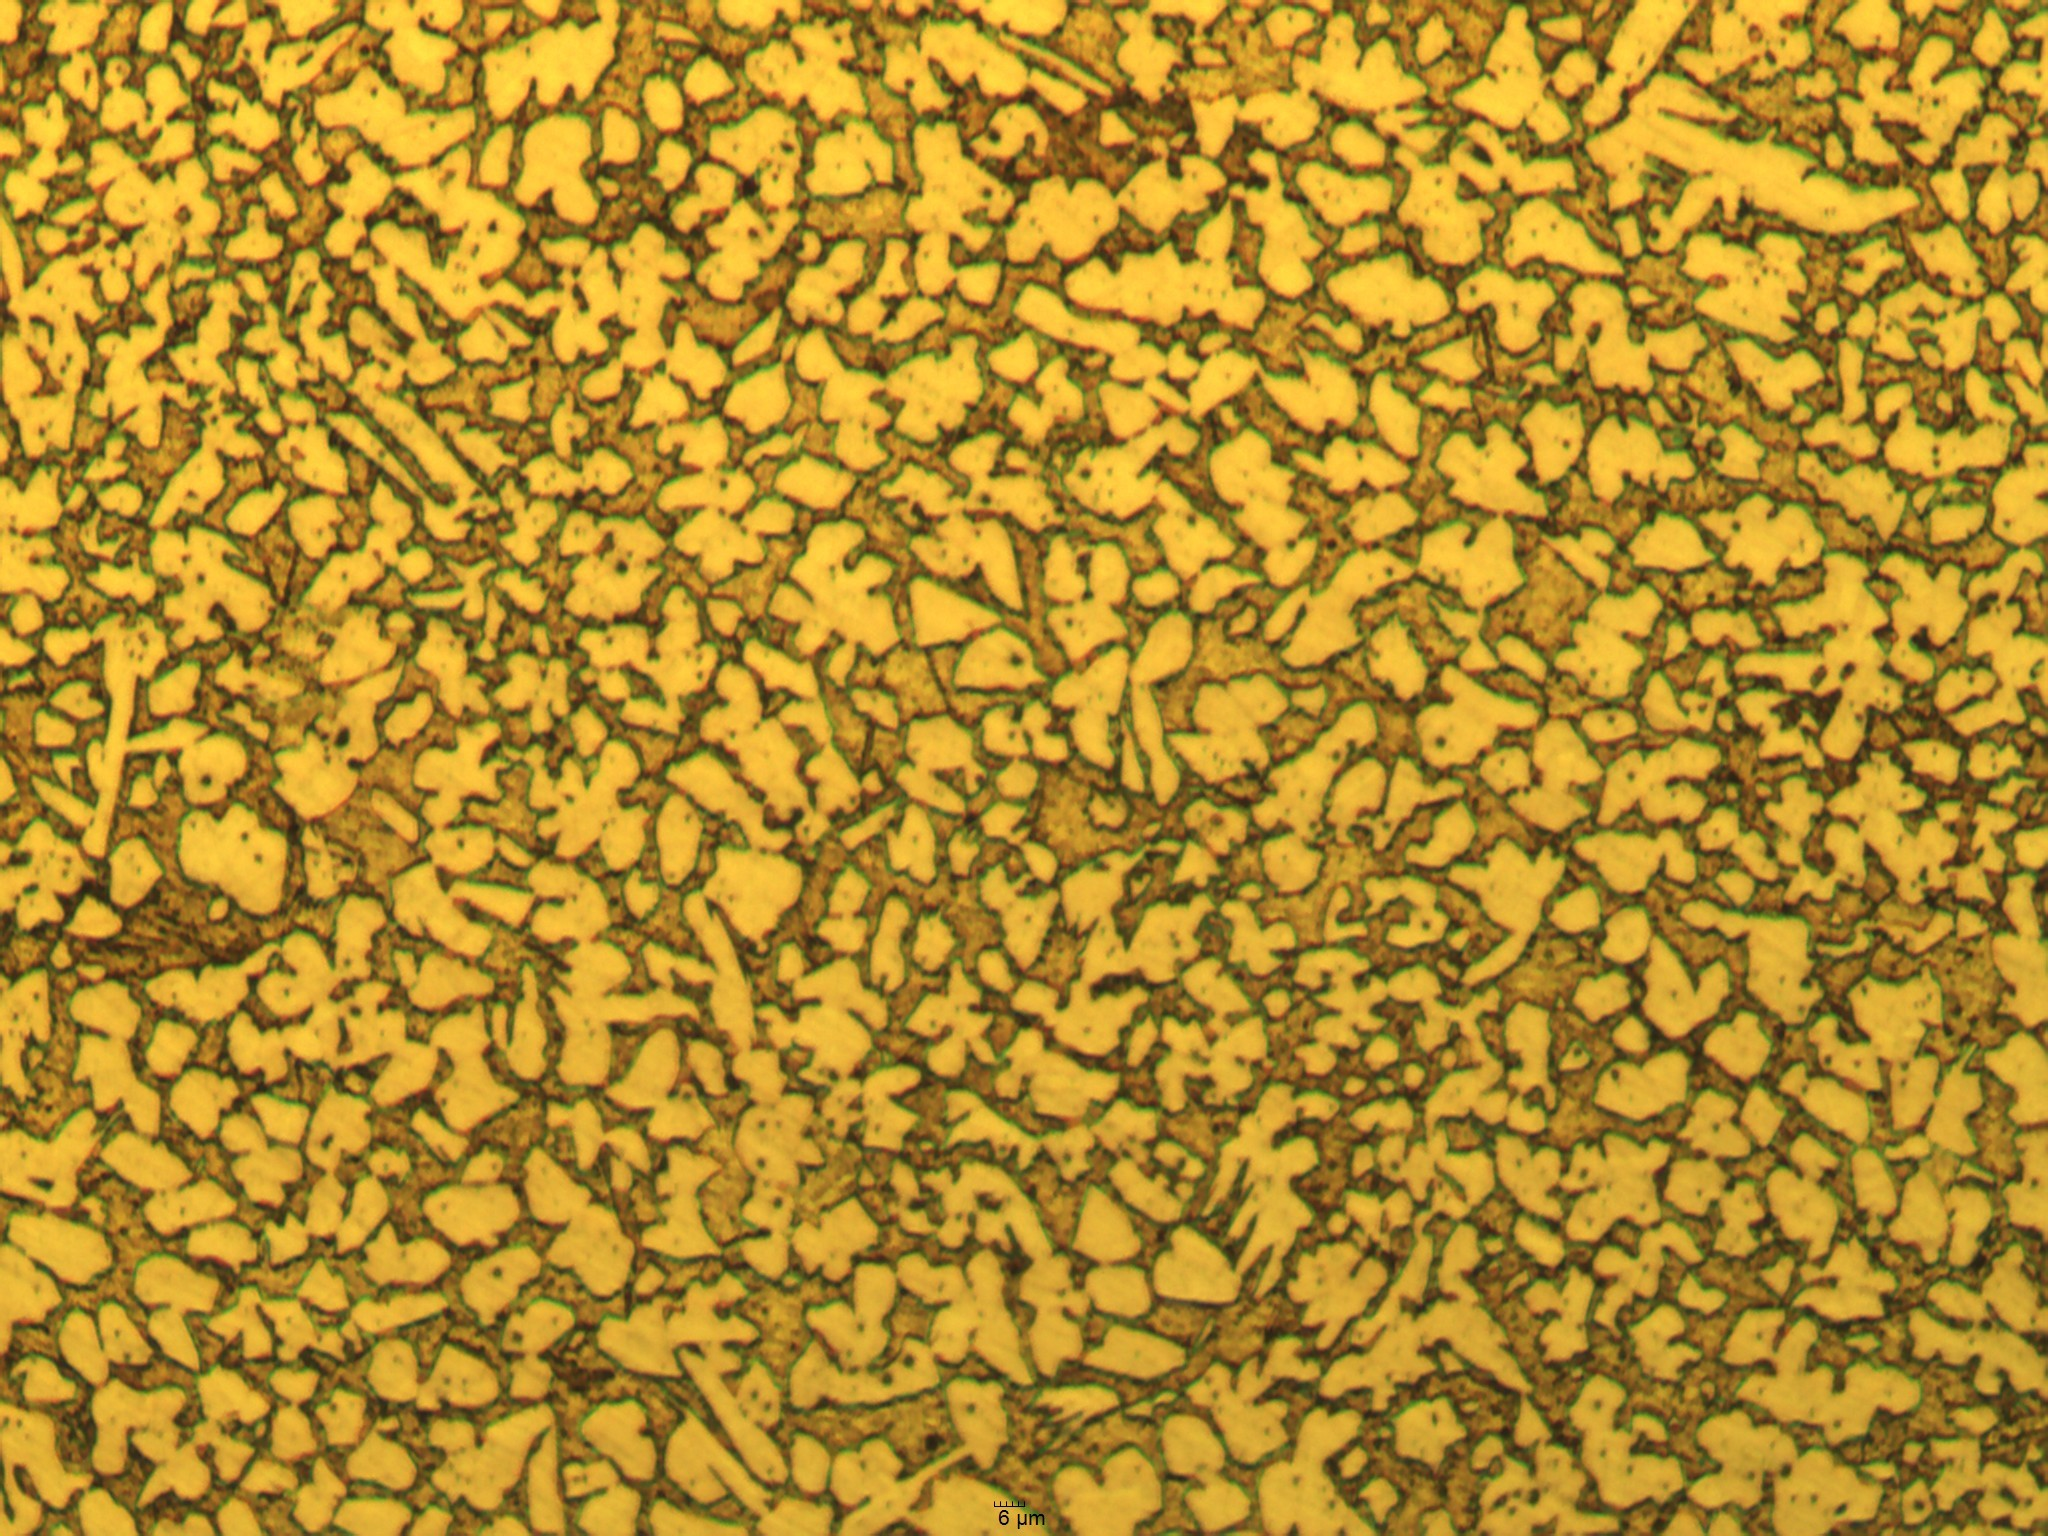
\includegraphics[scale=0.1]{Me_1Sch_25s_10x_001.jpg}
\captionof{figure}{Messing, 1.Ätzung, 10fach}
\end{minipage}
\begin{minipage}{0.1\textwidth}\centering
\[\]
\end{minipage}
\begin{minipage}{0.45\textwidth}\centering
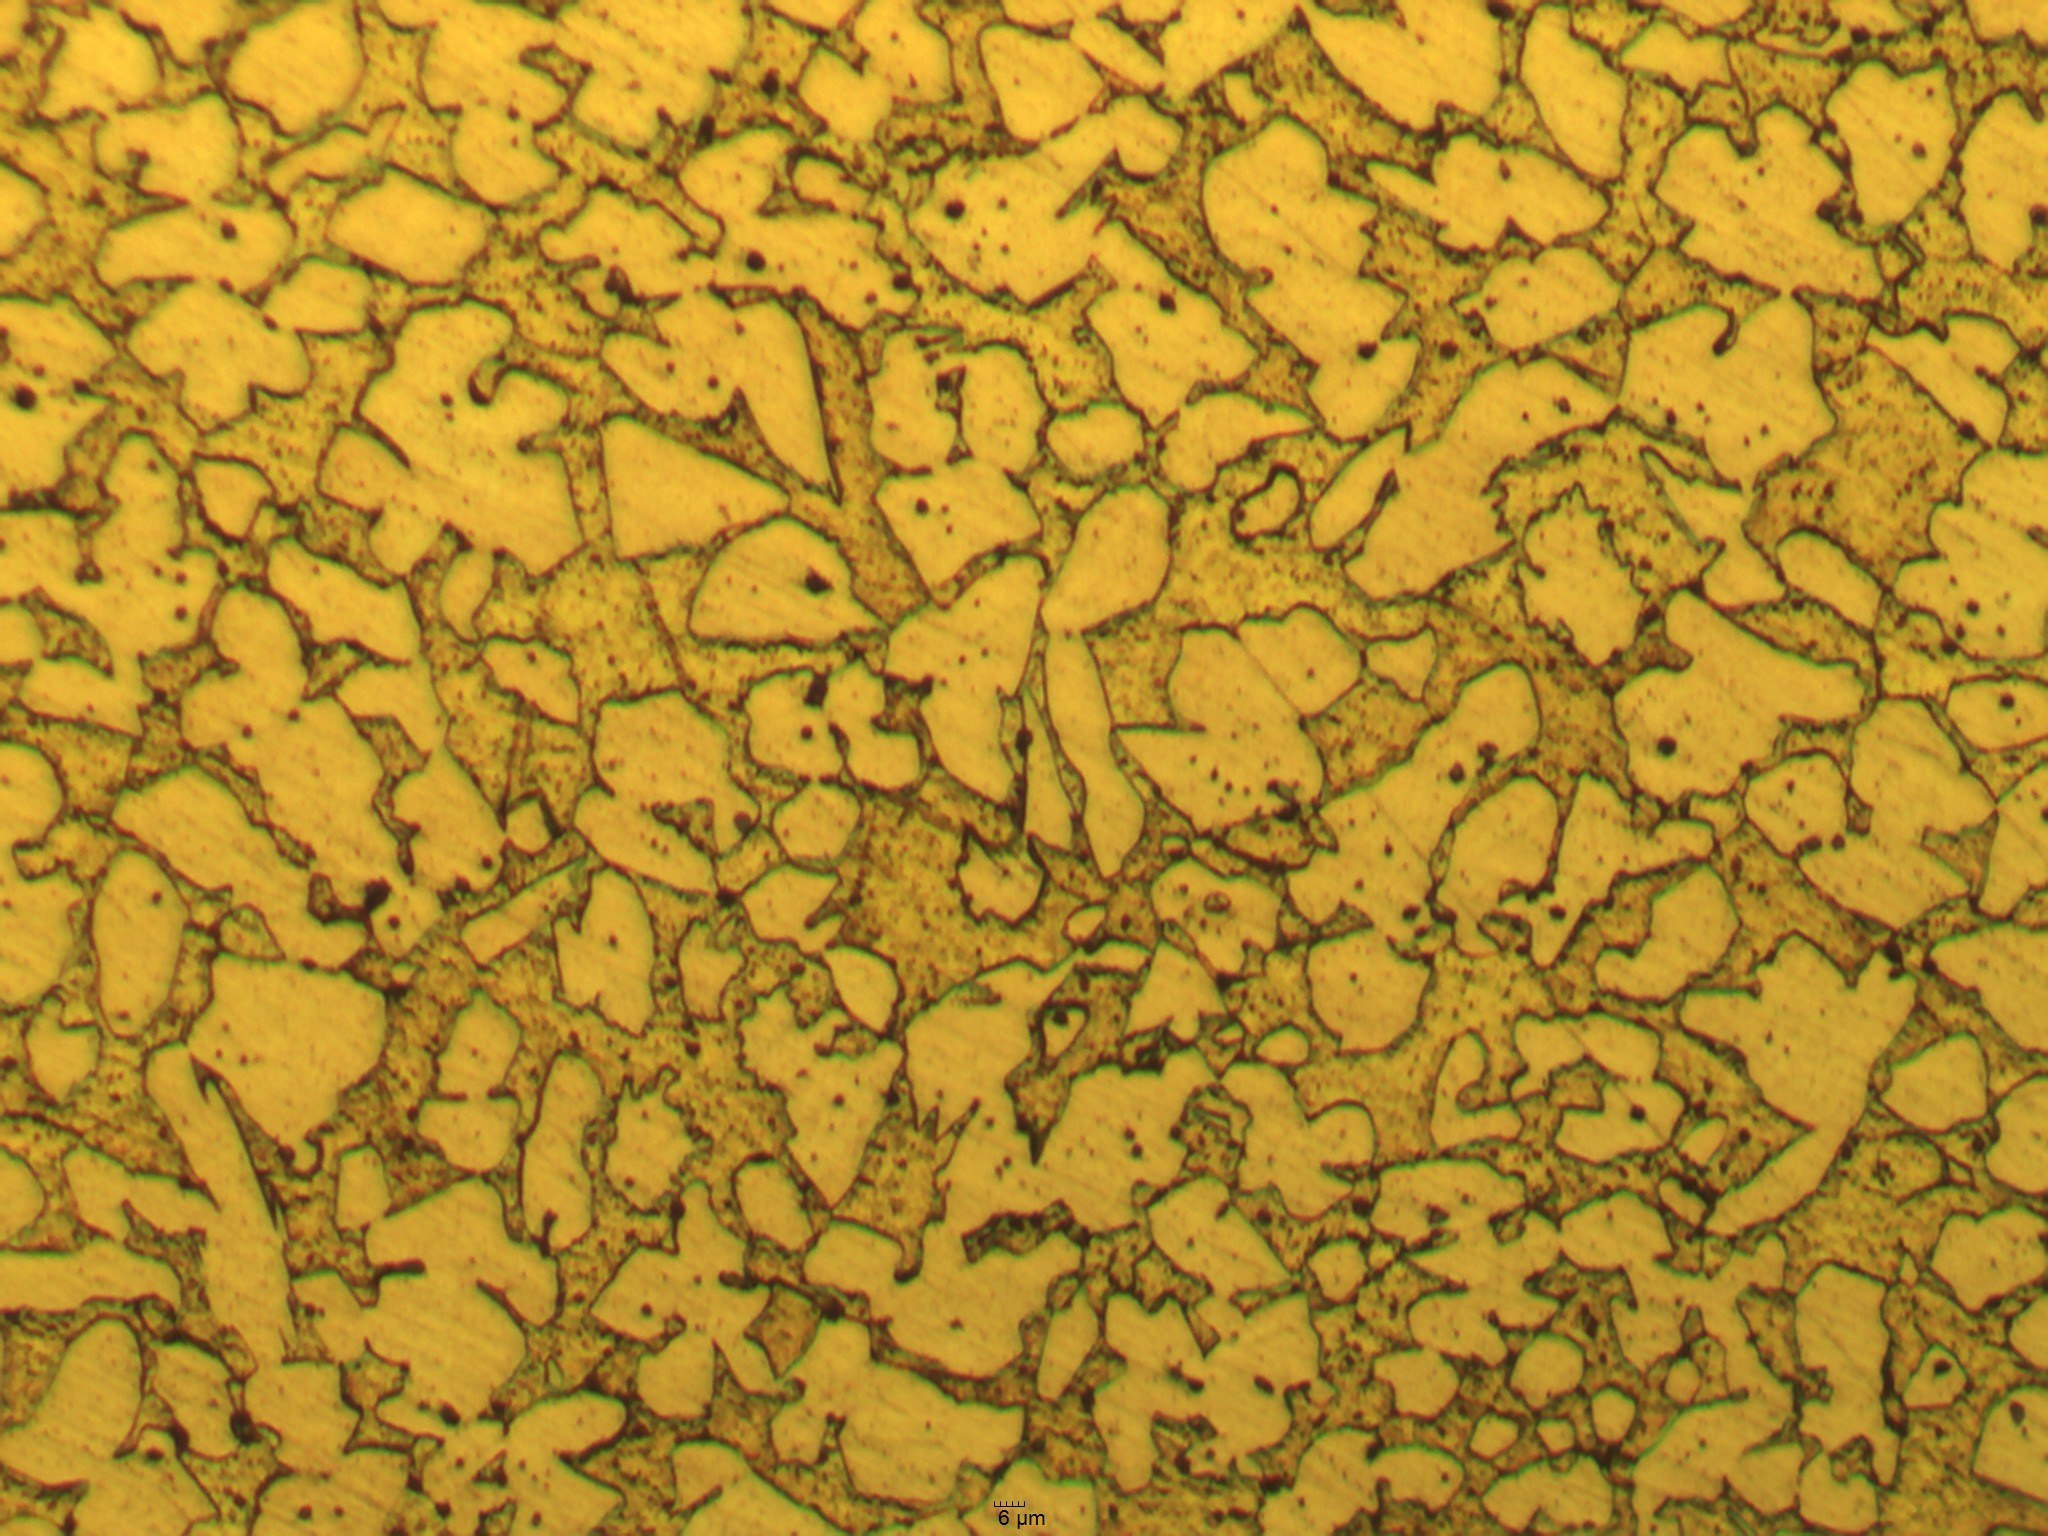
\includegraphics[scale=0.1]{Me_1Sch_25s_20x_001.jpg}
\captionof{figure}{Messing, 1.Ätzung, 20fach}
\end{minipage} \\\\\\
\begin{minipage}{0.45\textwidth}\centering
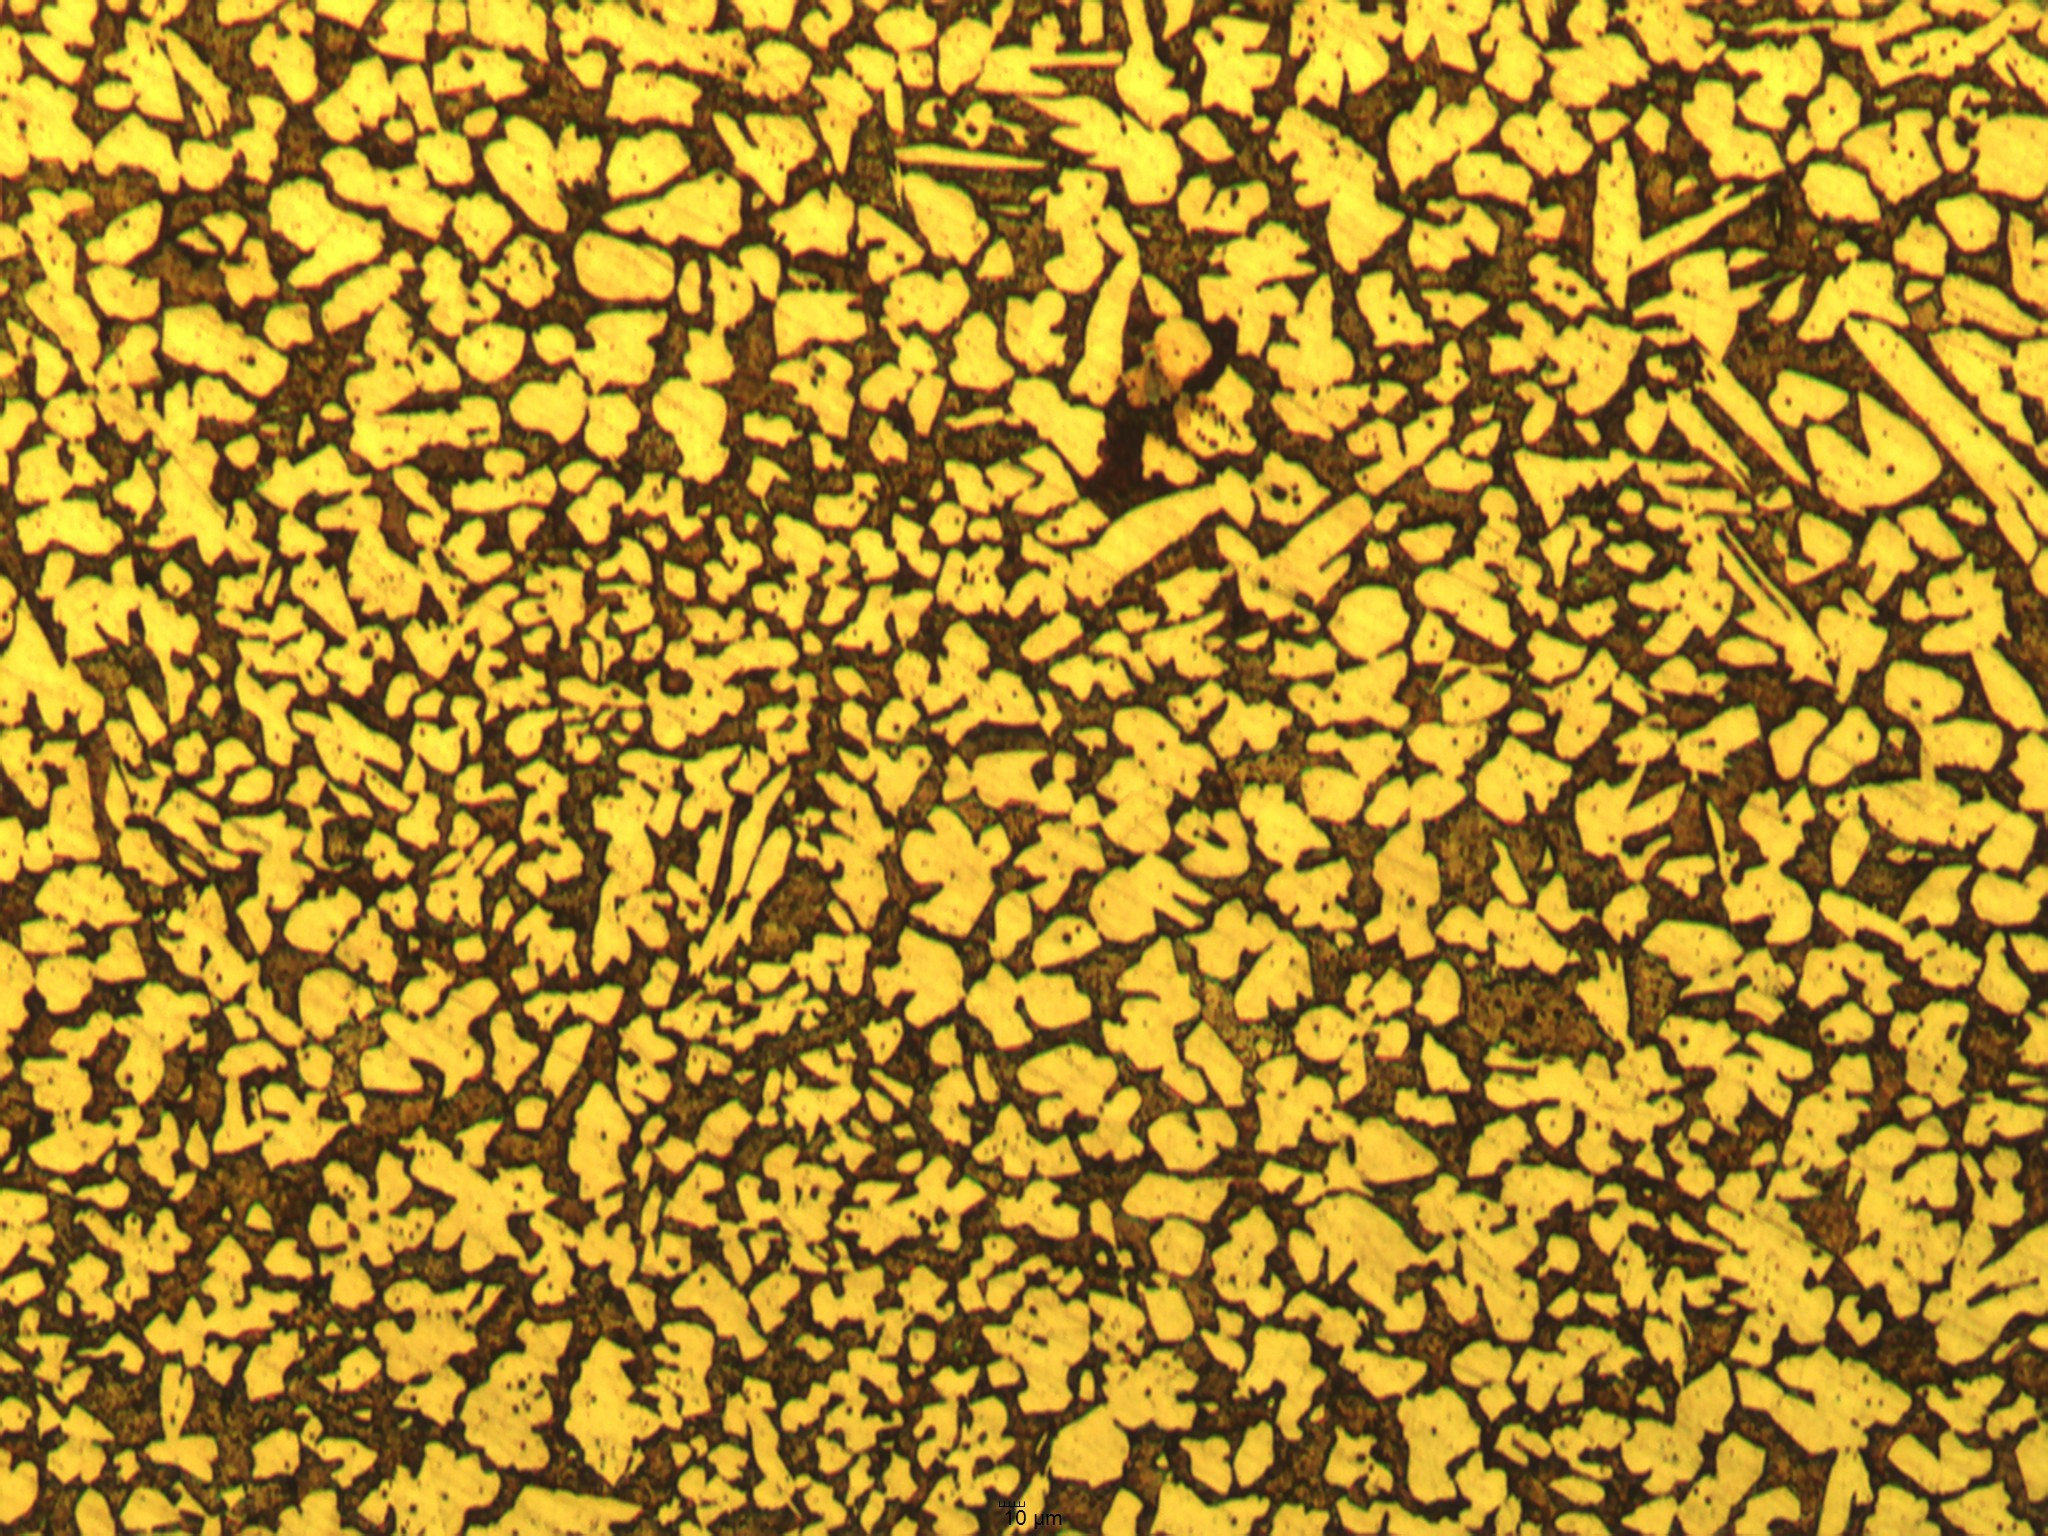
\includegraphics[scale=0.1]{Me_2Sch_5s_10x_001.jpg}
\captionof{figure}{Messing, 2.Ätzung, 10fach}
\end{minipage}
\begin{minipage}{0.1\textwidth}\centering
\[\]
\end{minipage}
\begin{minipage}{0.45\textwidth}\centering
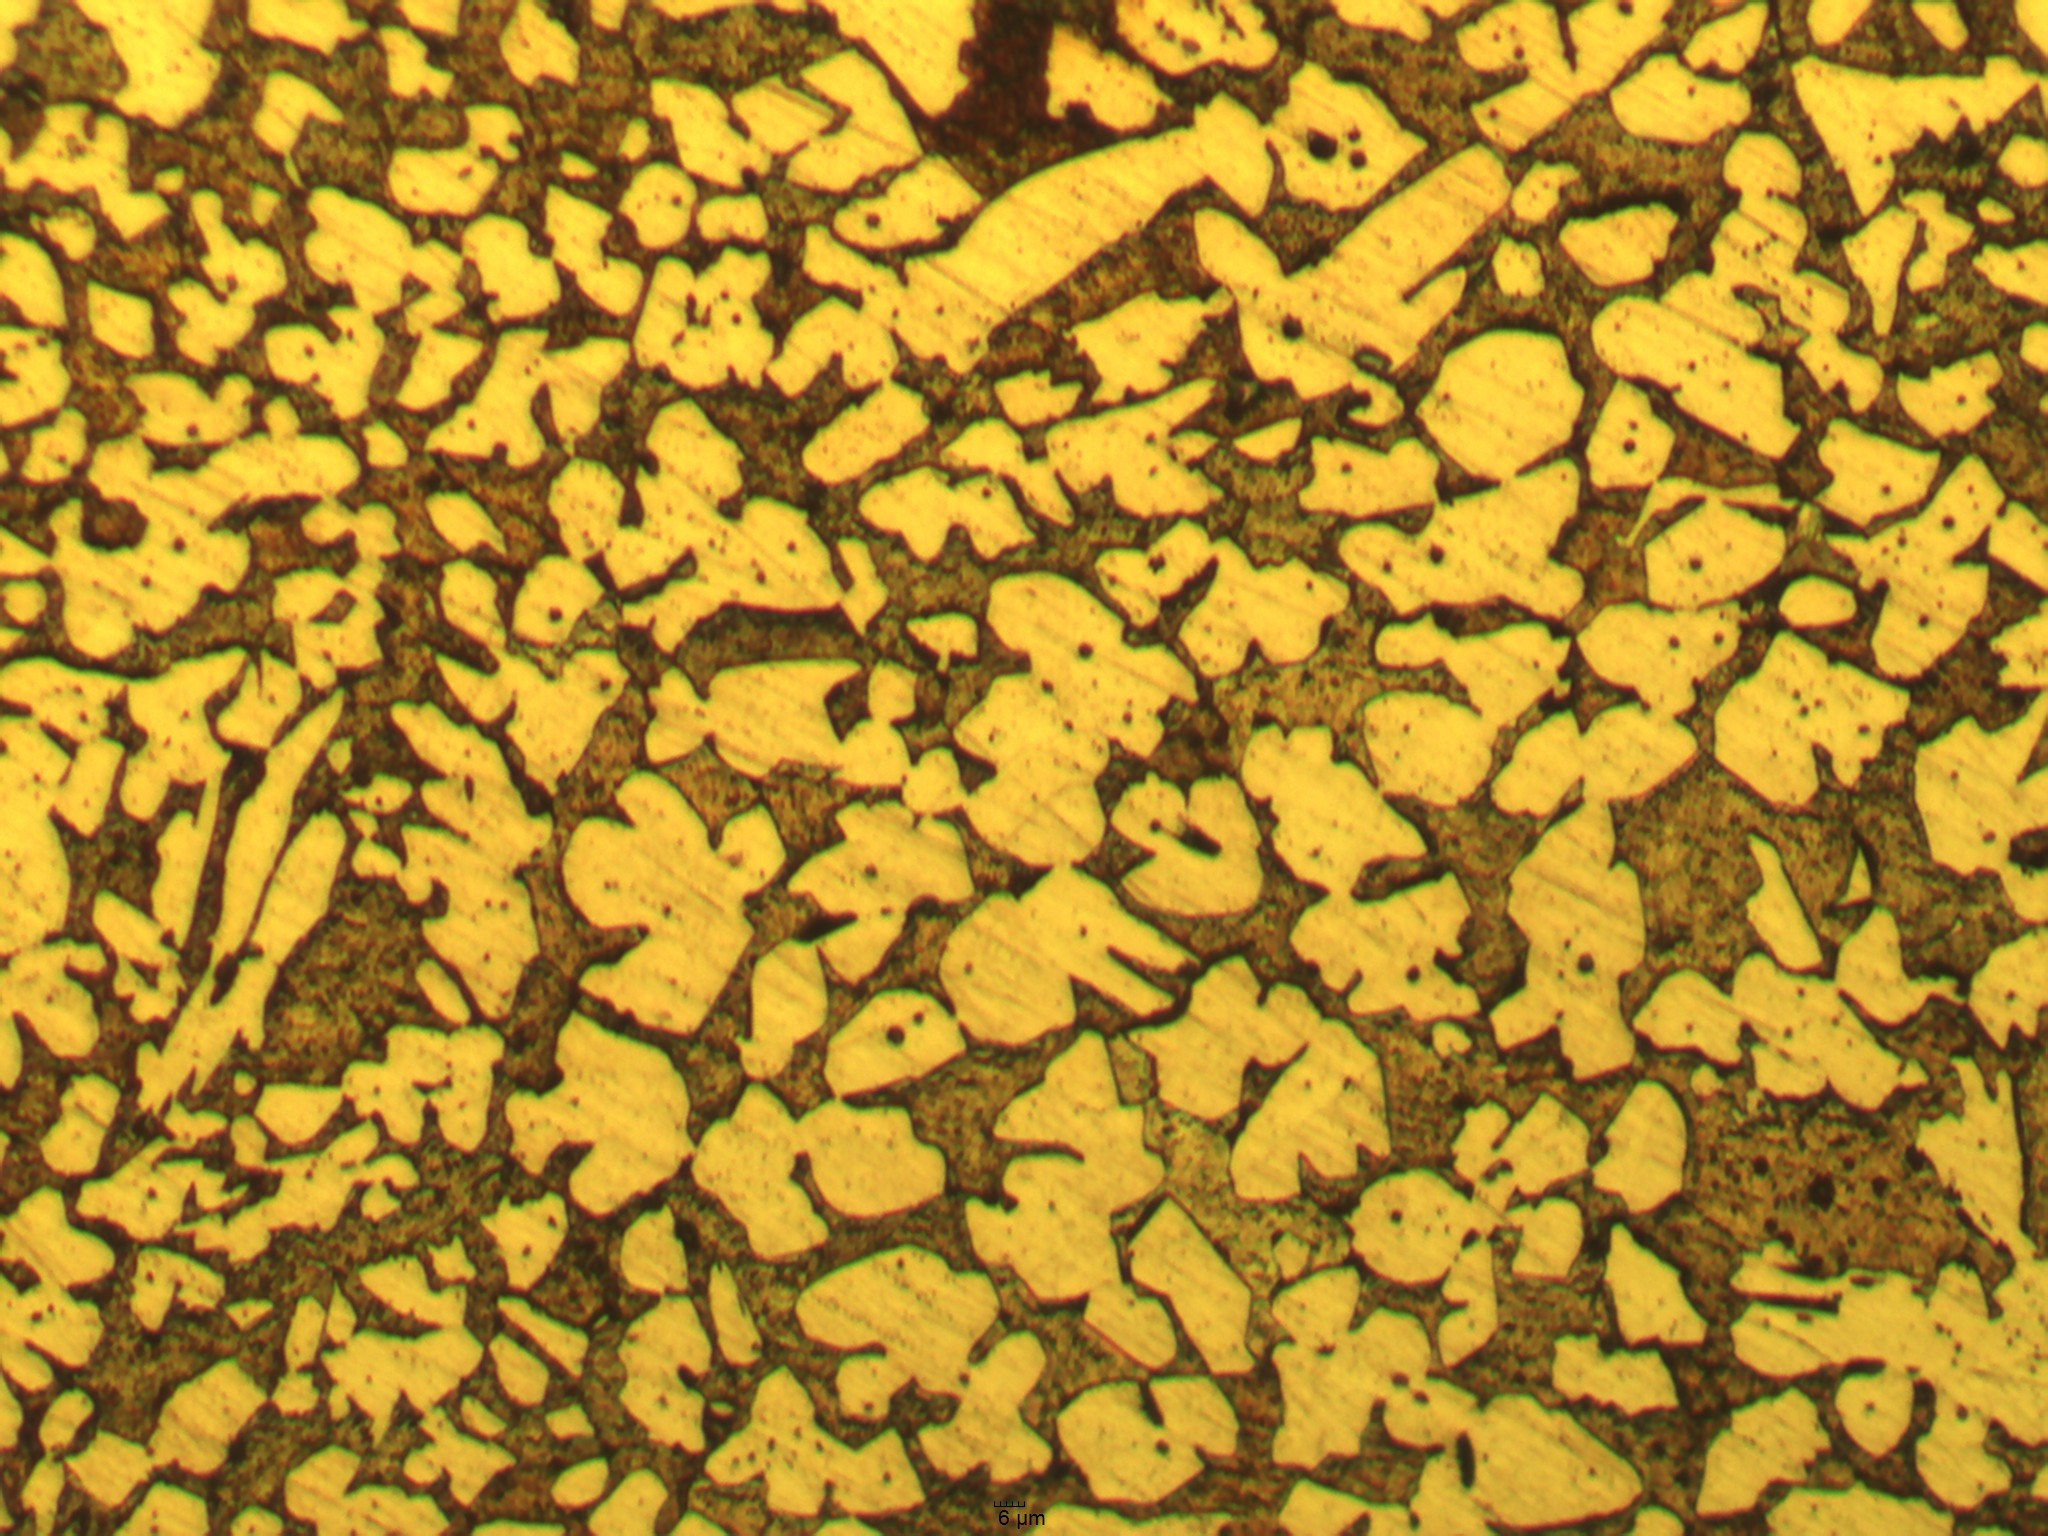
\includegraphics[scale=0.1]{Me_2Sch_5s_20x_001.jpg}
\captionof{figure}{Messing, 2.Ätzung, 20fach}
\end{minipage} 
\newpage
Das durch Ätzen herausgelöste $\beta$-Messing ist also für die dunklen Bereiche und das $\alpha$-Messing ist für die hellen Bereiche in den Abbildungen 12 bis 15 verantwortlich. 
\\
Für Stahl sehen die Abbildungen folgendermaßen aus:
\\\\\\
\begin{minipage}{0.45\textwidth}\centering
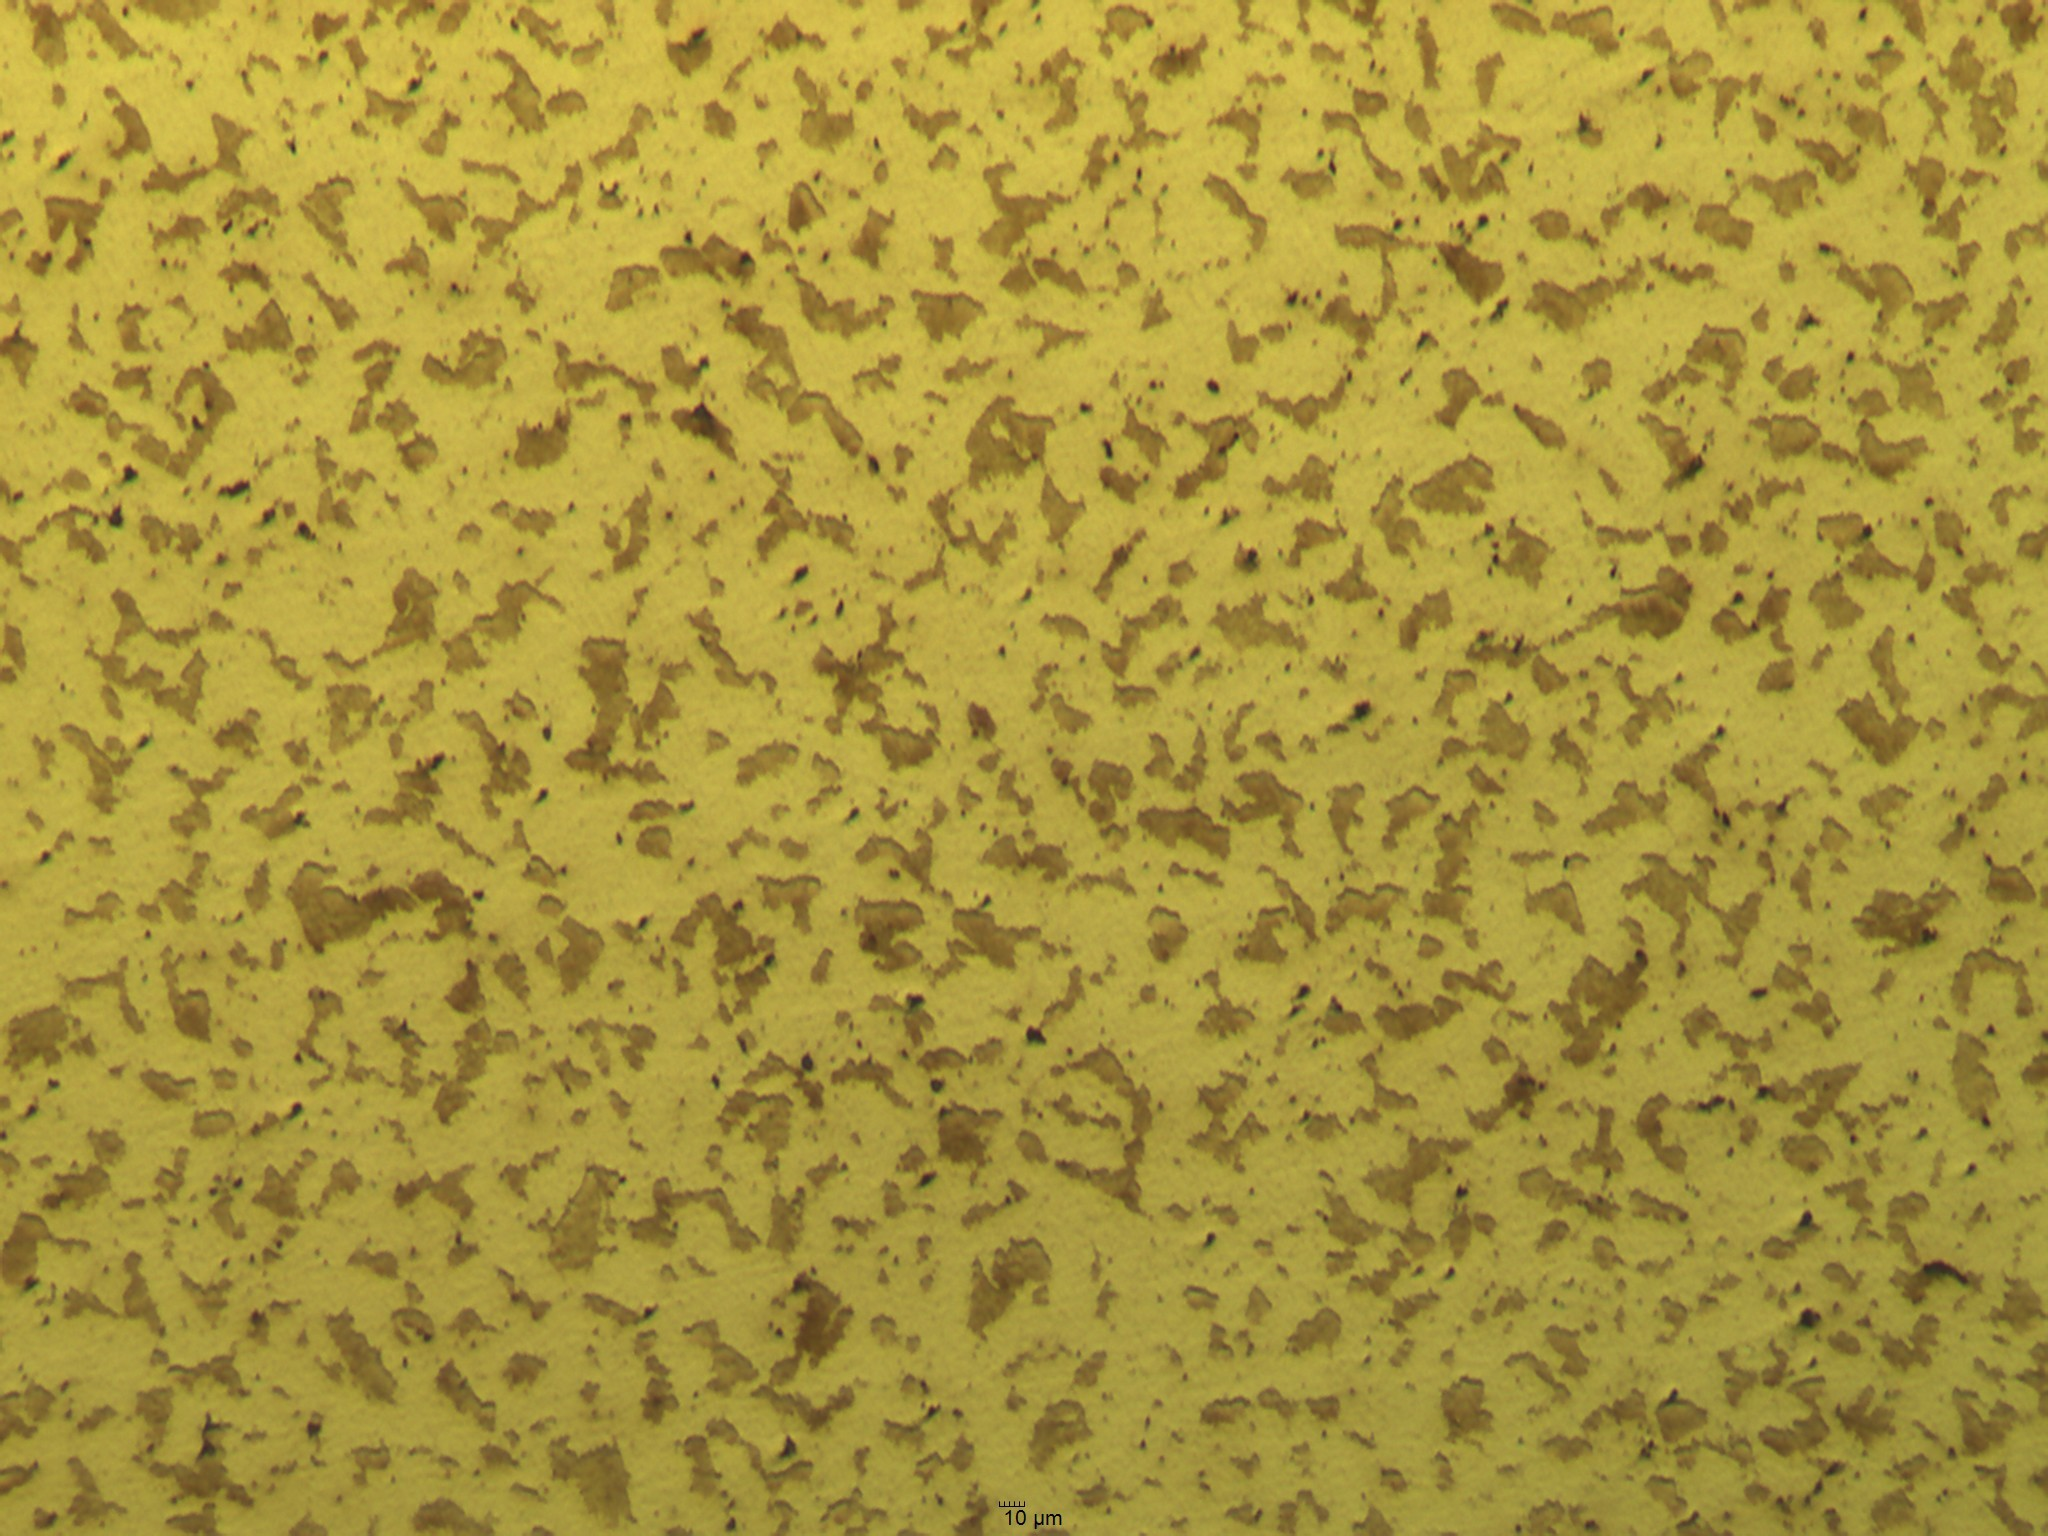
\includegraphics[scale=0.1]{St_1Sch_5s_10x_001.jpg}
\captionof{figure}{Stahl, 1.Ätzung, 10fach}
\end{minipage}
\begin{minipage}{0.1\textwidth}\centering
\[\]
\end{minipage}
\begin{minipage}{0.45\textwidth}\centering
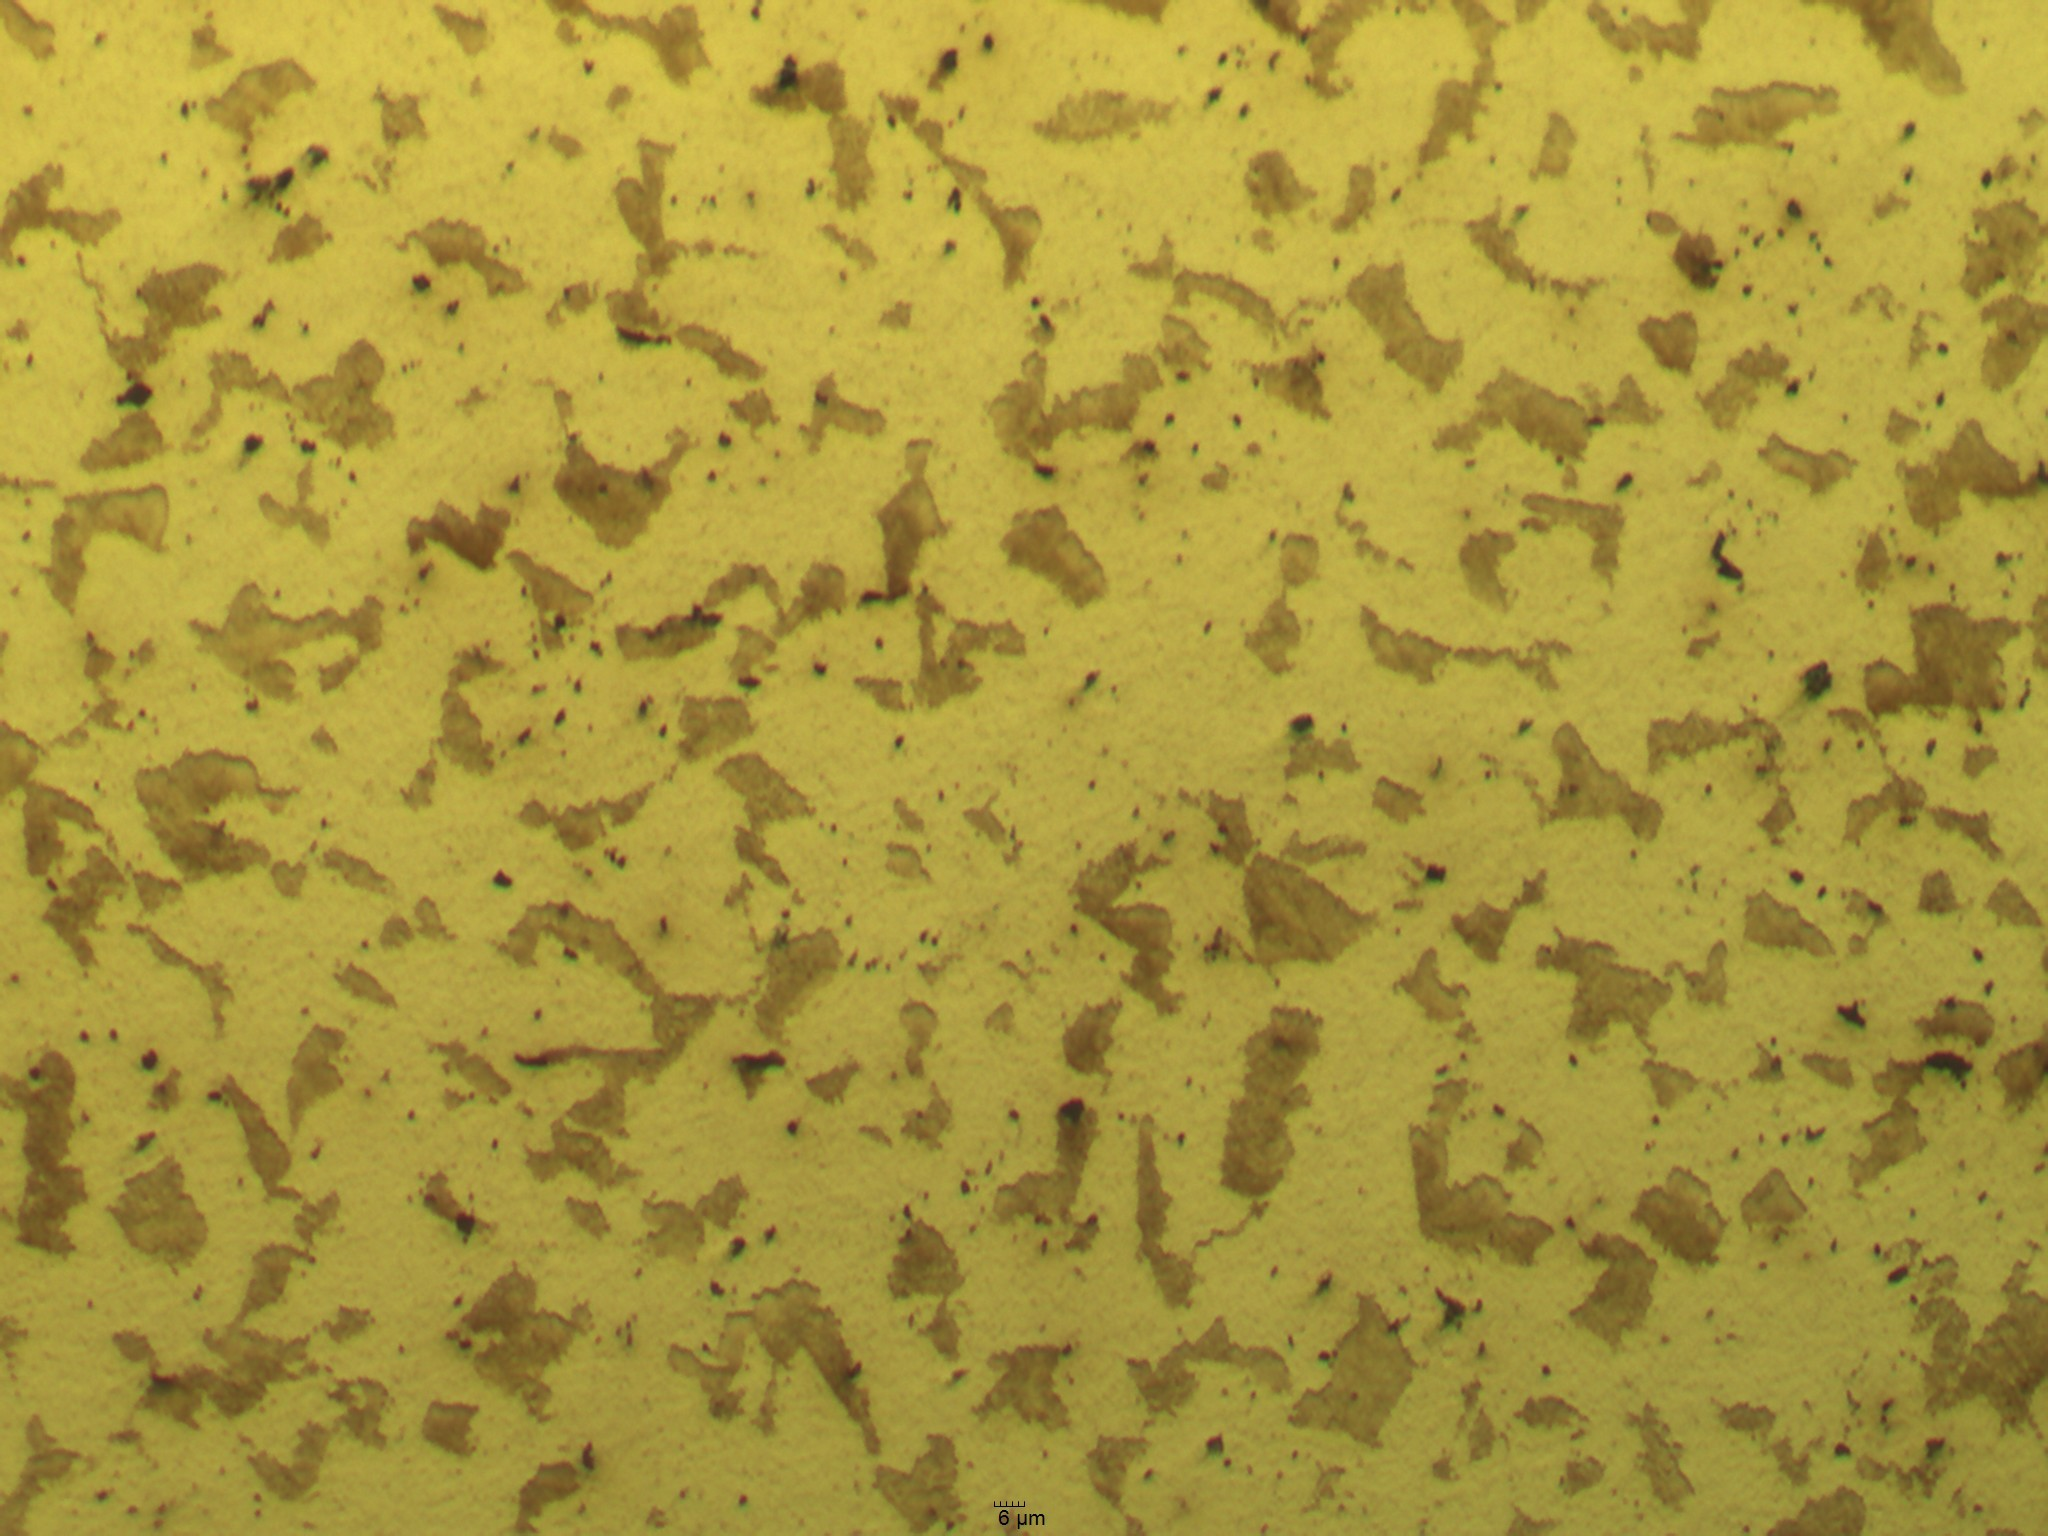
\includegraphics[scale=0.1]{St_1Sch_5s_20x_001.jpg}
\captionof{figure}{Stahl, 1.Ätzung, 20fach}
\end{minipage} \\\\

\begin{minipage}{0.45\textwidth}\centering
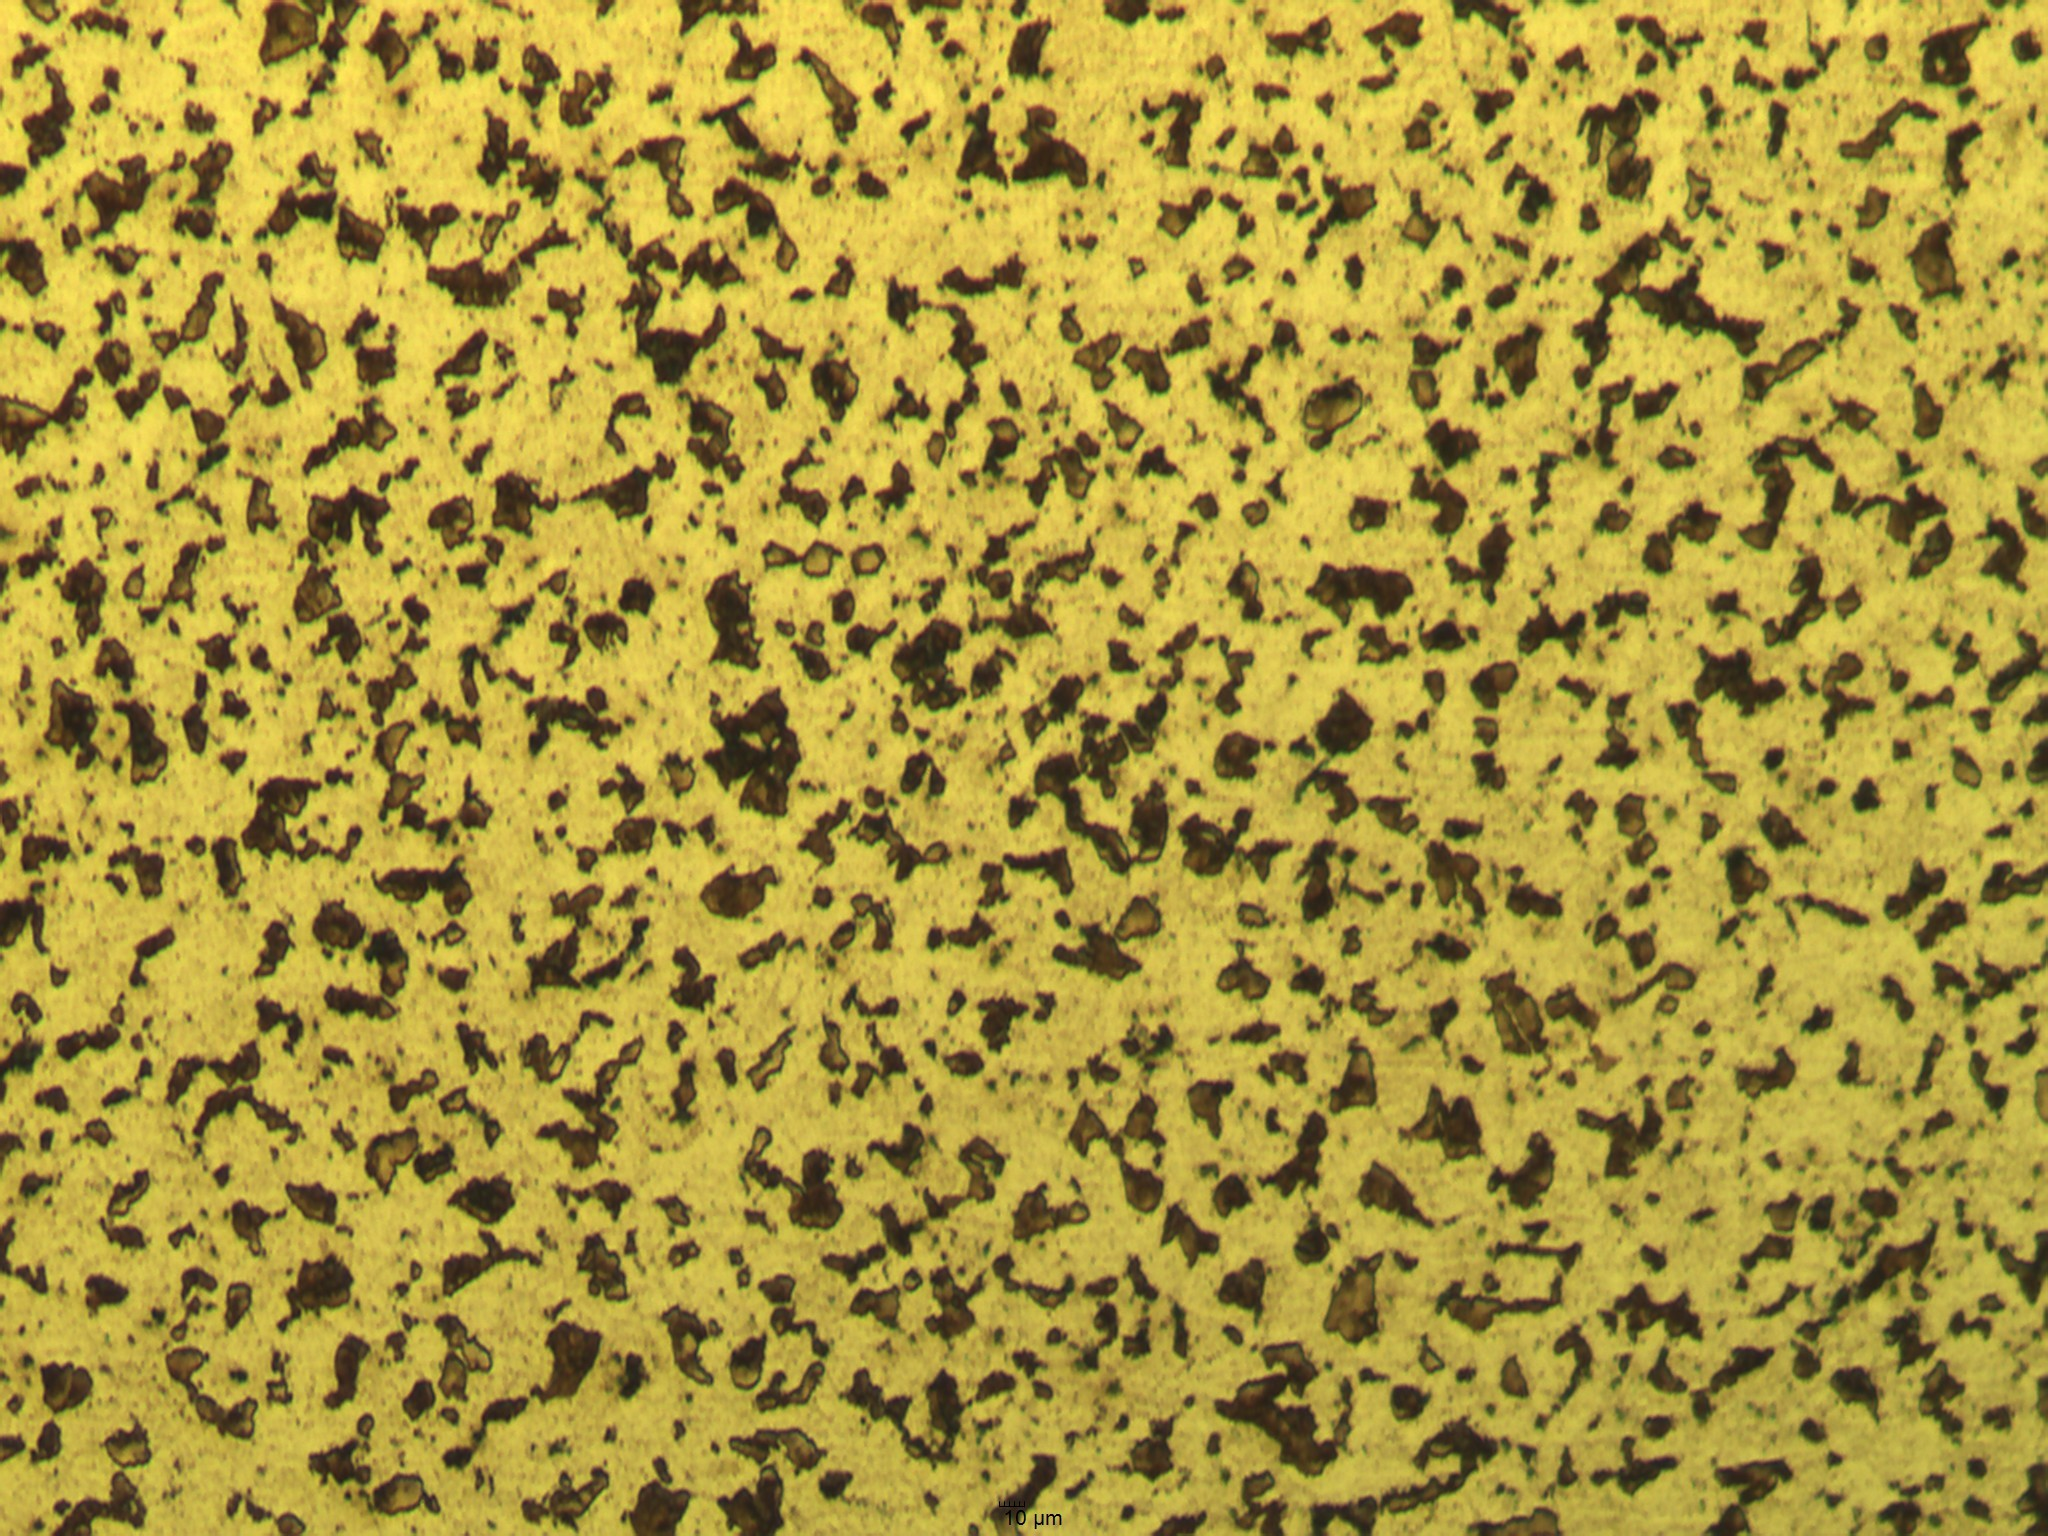
\includegraphics[scale=0.1]{St_2Sch_5s_10x_001.jpg}
\captionof{figure}{Stahl, 2.Ätzung, 10fach}
\end{minipage}
\begin{minipage}{0.1\textwidth}\centering
\[\]
\end{minipage}
\begin{minipage}{0.45\textwidth}\centering
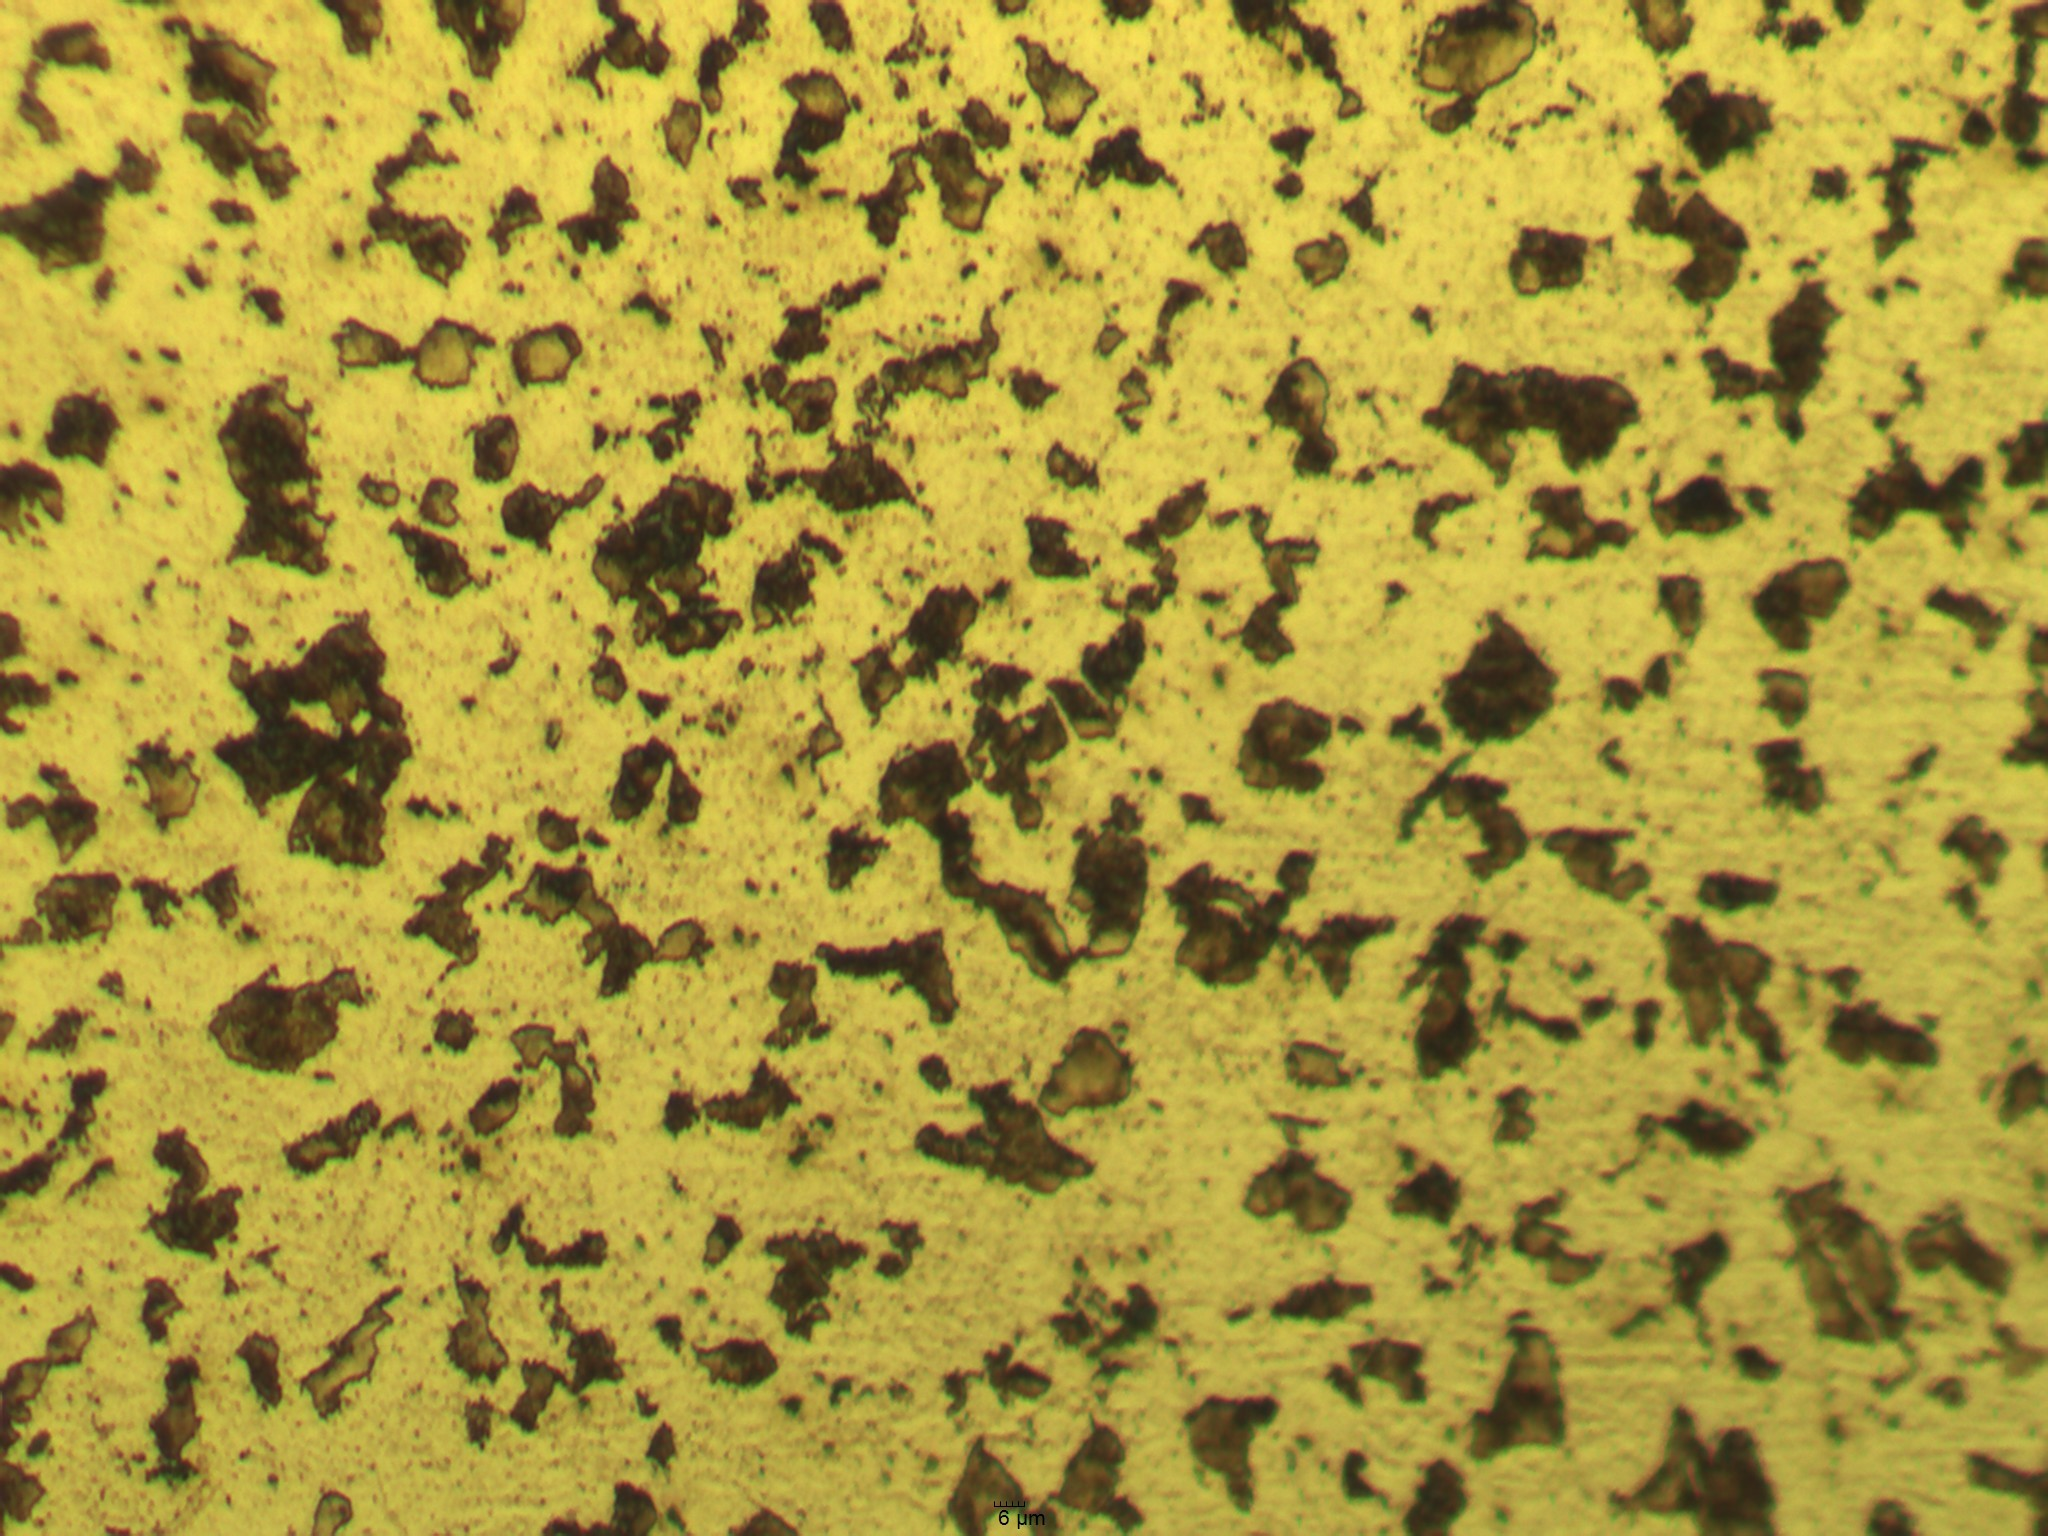
\includegraphics[scale=0.1]{St_2Sch_5s_20x_001.jpg}
\captionof{figure}{Stahl, 2.Ätzung, 20fach}
\end{minipage} \\\\\\
Für Stahl ist der herausgelöste Perlit für die dunklen Stellen und der Ferrit für die hellen Stellen verantwortlich.


\newpage
\section{Auswertung}
\subsection{Zur verwendeten Methode}
Wie in der theoretischen Vorbetrachtung erwähnt, besteht die Strategie für die Auswertung der Bilder jeweils darin, durch Ermitteln der hellen und dunklen Flächen auf die Volumenanteile der jeweils interessierenden Phase zu schließen. Anschließend ist es durch Kenntnis von Dichten und chemischer Zusammensetzung der Phase möglich, auf alle anderen Größen zu schließen. Die Hauptaufgabe besteht also im wesentlichen darin, die Flächenanteile zu erhalten. Dafür gibt es verschiedene stereologische Methoden. Wir haben folgende Variante genutzt:
\begin{enumerate}
\item Die aufgenommenen Bilder wurden zunächst in Graustufen konvertiert. Da die einzelnen Phasen jeweils helle und dunkle Bereiche bilden, ergibt sich die Schwierigkeit, dass man bei der Auswertung Farbbereiche festlegen müsste. Durch umwandeln in Graustufen reduziert sich die Einteilung der Bereiche auf den Hell-Dunkel-Kontrast anstatt auf Bereiche für rot, grün und blau, was die Auswertung einfacher macht.
\item Mithilfe des Moduls "PIL" (Python Image Library) können Bilder von der Sprache Python gelesen werden. Gleichzeitig ermöglicht das Modul die Umwandlung des Bildes in ein Array von Zahlen: Jedem Pixel wird dabei eine Zahl von 0 (ganz weiß) bis 255 (ganz schwarz) zugeordnet. Diese wurden anschließend durch Division mit 255 auf den Bereich zwischen 0 und 1 normiert.
\item Nachdem das Bild in Zahlen umgewandelt wurde, können die Daten statistisch ausgewertet werden. Mithilfe eines einfachen selbst geschriebenen Programms wurden alle Pixel gezählt und ein Histogramm mit je 50 Intervallen erzeugt, welches die statistische Verteilung der Hell-Dunkel-Werte widerspiegelt. Die Verteilung hatte jeweils nahe den Rändern zwei ausgeprägte Maxima und dazwischen ein Minimum. An diesem Minimum wurde jeweils die Grenze zwischen den hellen und dunklen Bereichen festgelegt. Durch diese statistische Analyse wird eine Willkür bei der Festlegung der Bereiche für Hell und Dunkel weitgehend vermieden.
\item Es wurden dann alle Pixel gezählt, die in die beiden Bereiche fallen und damit deren relative Häufigkeit errechnet. Diese bilden dann direkt die Volumenanteile der jeweiligen Phase an der Probe im betrachteten Bereich. Damit der so ermittelte Wert repräsentativ für die gesamte Probe ist, wurde das Bild mit der kleinsten Vergrößerung (zehnfach) gewählt. Dadurch wird ein ausreichend großer Bereich untersucht, der Mischkristalle in verschiedenen Größen enthält.
\item Das Histogramm bietet außerdem eine Möglichkeit, die statistischen Unsicherheiten der relativen Häufigkeiten abzuschätzen. Da das Histogramm eine Zählstatistik ist, hat man bei \(n\)-vielen Treffern in einem gegebenen Intervall eine Unsicherheit von \(\Delta n \approx \pm\sqrt{n}\) nach \textsc{Poisson}. Da sich die die relativen Häufigkeiten bei \(N\) Pixeln insgesamt durch 
\[h_{\mathrm{rel.}} = \frac{n}{N}\] 
berechnen, ergibt sich die Unsicherheit der relativen Häufigkeit mittels \textsc{Gauß}scher Fehlerfortpflanzung zu
\[\Delta h_{\mathrm{rel.}} = \sqrt{\left(\frac{\partial h_{\mathrm{rel.}}}{\partial n} \Delta n \right)^2} = \sqrt{\left(\frac{1}{N}\sqrt{n}\right)^2} = \left|\frac{\sqrt{n}}{N}\right|\]
Bei \(n\) Pixeln im Intervall lautet also das Ergebnis für die jeweilige relative Häufigkeit
\[\underline{\underline{h_{\mathrm{rel.}} = \left(\frac{n}{N} \pm \frac{\sqrt{n}}{N} \right)}}\]
\item Es wurden dann die relativen Häufigkeiten aller Intervalle im Histogramm oberhalb der Grenze addiert und dem hellen Bereich zugeordnet. Bei der Addition addieren sich gemäß \textsc{Gauß}scher Fehlerfortpflanzung die Unsicherheiten:
\[\underline{\underline{h_{\mathrm{rel.}}^{\mathrm{(hell)}} = \left(\sum_{\mathrm{hell}}\frac{n^{\mathrm{(hell)}}}{N} \pm \sum_{\mathrm{hell}}\frac{\sqrt{n^{\mathrm{(hell)}}}}{N} \right)}}\]
Mit dem Bereich unterhalb der Grenze (dunkel) wurde völlig analog verfahren. 
\end{enumerate}

\subsection{Silizium}
Hier soll die Auswertung eher qualitativ erfolgen. Zunächst kann man feststellen, wie sich die verschiedenen Schritte auf die Oberflächenstruktur ausgewirkt haben:
\begin{itemize}
\item Nach dem Läppen war die Oberfläche mattgrau. Mit jedem Ätzschritt wurde die Probe immer stärker glänzend. Es ließen sich also auch deutliche makroskopische Veränderungen erkennen.
\item Beim ersten Ätzvorgang wurde die anfangs nur grob geschliffene Fläche chemisch abgetragen. Unter dem Mikroskop erkennt man eine hügelige Oberfläche. Bei der kleinsten Vergrößerung (12.5fach), siehe Abbildung 6, lassen sich einzelne Silizium-Körnchen gut erkennen.
\item Der zweite Ätzschritt hat die Oberfläche chemisch poliert. Dadurch hat sich die Zahl der Hügel deutlich reduziert, weshalb die stärkere Vergrößerung verwendet wurde. Man kann in Abbildung 8 bereits erste kleinere Ätzgrübchen erkennen.
\item Im letzten Schritt wurden die Ätzgrübchen sehr deutlich herausgebildet. Sie formen unterschiedliche und sehr interessante Strukturen, von denen die besten Aufnahmen zusammengestellt wurden. Dies sind die Abbildungen 9 bis 11.
\end{itemize}
Die Ätzgrübchen bilden perfekte gleichseitige Dreiecke. Das bestätigt, dass die untersuchte Ebene die (111) Ebene ist. Insgesamt waren die Ätzgrübchen auf eher kleinere Bereiche im Kristall lokalisiert, die in höchster Vergrößerung (50fach) untersucht wurden. Die auf den gesamten Kristall betrachtet geringe Dichte an Ätzgrübchen lässt auf ein weitgehend gleichmäßiges Wachstum des Kristalls schließen. Dies rechtfertigt die Bezeichnung als Einkristall mit Versetzungen im Vergleich etwa zum später folgenden Stahl und Messung, die sehr viele Mischkristalle enthalten.\\\\
Anhand von Abbildung 10 kann die Versetzungsdichte berechnet werden. Die Anzahl der Dreiecke beträgt $N_{\Delta} = 151$. Als Unsicherheit der Zählung wird $\Delta N_{\Delta} = 10$ angenommen, da es sehr schwierig ist genau zu zählen. Die in der Abbildung abgebildete Fläche ist $A = 0,019$ mm$^2$. Die Versetzungsdichte $\rho$ und ihre Unsicherheit $\Delta \rho$ sind somit:
\begin{align}
\rho &= \frac{N_{\Delta}}{A} \approx 7947,37 \frac{1}{\text{mm}^2} \\
\Delta \rho &= \frac{\Delta N_{\Delta}}{A} \approx 526,32 \frac{1}{\text{mm}^2}
\end{align}
Das Endergebnis für die Versetzungsdichte in Abbildung 10 ist dementsprechend:
\begin{align*}
\underline{\underline{\rho \pm \Delta \rho = (7947,37 \pm 526,32) \, \frac{1}{\text{mm}^2}}}
\end{align*}
\subsection{Kohlenstoffanteil im Stahl}
Für die Berechnung des Kohlenstoffanteils im Stahl werden die Bilder für den ersten Ätzschritt von Stahl bei 10-facher Vergrößerung (Abbildung 16) und für den 2. Ätzschritt bei 10-facher Vergrößerung (Abbildung 18) verwendet.
\subsubsection{Erster Ätzschritt}
Gegeben waren folgende Werte für den Volumenanteil von Ferrit und Zementit im Perlit:
\begin{align*}
V(\text{Ferrit}) &:= V(\text{Fe}) \,\,\,\,\,\,\,\,\,= 85,5 \, \text{Vol}\% \\
V(\text{Zementit}) &:= V(\text{$Fe_{3}C$}) = 13,5 \,  \text{Vol}\%
\end{align*}
Außerdem lassen sich aus der Anleitung für Stahl die Werte der Dichten für Ferrit und Zementit herauslesen:
\begin{align*}
\rho(\text{Fe}) &= 7,86 \frac{\text{g}}{\text{cm}^3} \\
\rho(\mathrm{Fe}_{3}\mathrm{C}) &= 7,4 \frac{\text{g}}{\text{cm}^3}
\end{align*}
Daraus ergibt sich über folgende Gleichung das Masseprozent des Zementits bezogen auf Perlit aus den Volumenprozenten:
\begin{align*}
G_{\mathrm{A}} = \frac{100}{1 + \frac{V_{\mathrm{B}} \rho_{\mathrm{B}}}{V_{\mathrm{A}} \rho_{\mathrm{A}}}}
\end{align*}
Hierbei bezeichnet dann A Zementit ($\mathrm{Fe}_{3}\mathrm{C}$) und B Ferrit (Fe). Somit ergibt sich:
\begin{align*}
G_{\mathrm{Fe}_{3}\mathrm{C}} = 12,81 \, \text{Gew}\%
\end{align*}
Da bekannt ist, welchen Massenanteil Zementit im Perlit ausmacht, kann man nun berechnen, wie groß der Massenanteil an Zementit in der gesamten Probe ist. Dazu wird der aus dem Bild ermittelte Volumenanteil an Perlit verwendet. Dieser lag im 1. Ätzschritt bei $V(\text{Perlit}) = 11,4 \, \text{Vol}\%$. Daraus folgt:
\begin{align*}
G_{\mathrm{Fe}_{3}\mathrm{C}}^{\mathrm{gesamt}} &= G_{\mathrm{Fe}_{3}\mathrm{C}} \cdot V(\text{Perlit}) \\
&= 12,81 \cdot 0,114 \, \text{Gew}\% \\
&= 1,46 \, \text{Gew}\%
\end{align*}
Um nun den Massenanteil an Kohlenstoff zu bestimmen, muss aus der Anleitung zu Stahl verwendet werden, dass Zementit $6,67 \%$ Kohlenstoff enthält. Somit ist der Gesamtmassenanteil an Kohlenstoff der Probe gegeben durch:
\begin{align*}
G_{\text{C}} &= G_{\mathrm{Fe}_{3}\mathrm{C}}^{\mathrm{gesamt}} \cdot 6,67\% \\
&=1,46 \cdot 0,0667 \, \text{Gew}\% \\
&=0,097 \, \text{Gew}\%
\end{align*}
Diese Größe ist allerdings in Folge der Auswertung mit einem Programm fehlerbehaftet.
Die Unsicherheit für den Volumenanteil von Perlit beträgt:
\begin{align*}
\Delta V(\text{Perlit}) = 1,6 \, \text{Vol}\%
\end{align*}
Dies wirkt sich in folgender Form auf den Anteil an Kohlenstoff aus:
\begin{align*}
\Delta G_{\text{C}}&= \left | \frac{\partial G_{\text{C}}}{\partial V(\text{Perlit})} \cdot \Delta V(\text{Perlit}) \right | \\
&= 0,667 \cdot 0,1281 \cdot \Delta V(\text{Perlit}) \\
&= 0,014 \, \text{Gew}\%
\end{align*}
Man erhält also als Gesamtresultat für den Kohlenstoffanteil, bestimmt beim 1. Ätzschritt:
\begin{align*}
\underline{\underline{G_{\text{C}} \pm \Delta G_{\text{C}} = (0,097 \pm 0,014) \, \text{Gew}\%}}
\end{align*}

\subsubsection{Zweiter Ätzschritt}
Selbige Rechnung wurde nochmal für den 2. Ätzschritt (Abbildung 18) wiederholt. Hierbei ergaben sich aus dem Bild folgende Werte:
\begin{align*}
V(\text{Perlit}) &= 12,7 \, \text{Vol}\% \\
\Delta V(\text{Perlit})  &= 0,5 \, \text{Vol}\%
\end{align*}
Als Resultat für den Kohlenstoffanteil erhält man hier:
\begin{align*}
\underline{\underline{G_{\text{C}} \pm \Delta G_{\text{C}} = (0,109 \pm 0,004) \, \text{Gew}\%}}
\end{align*}
Es ist also zu erkennen, dass durch den zweiten Ätzschritt, in dem der Kontrast des Bildes nochmals erhöht wurde, sowohl die absolute Messunsicherheit, als auch die relative Messunsicherheit verringert werden konnten.

\subsection{Anteil vom Zink im Messing}
Für die Berechnung des Zinkanteils im Messing werden die Bilder für den ersten Ätzschritt von Messing bei 10-facher Vergrößerung (Abbildung 12) und für den 2. Ätzschritt bei 10-facher Vergrößerung (Abbildung 14) verwendet.
\subsubsection{Erster Ätzschritt}
Für diesen Teil der Auswertung sind die Atomprozente von Zink im $\alpha$- und $\beta$-Mischkristall gegeben:
\begin{align*}
\text{X}_{\text{Zn}}^{\alpha} &= 38 \, \text{At}\% \\
\text{X}_{\text{Zn}}^{\beta} &= 44,3 \, \text{At}\%
\end{align*}
Zudem sind die Atommassen von Kupfer und Zink bekannt:
\begin{align*}
\text{m}_{\text{Cu}} &= 63,546 \, \text{u} \\
\text{m}_{\text{Zn}} &= 65,38 \, \text{u}
\end{align*}
Durch folgende Umrechnungen ermittelt man daraus die jeweiligen Masseprozente des Zinks im $\alpha$- bzw. $\beta$- Messing:
\begin{align*}
\text{G}_{\alpha}^{\text{Zn}} &= \frac{100}{1+\frac{\text{X}_{\text{Cu}}^{\alpha} \cdot \text{m}_{\text{Cu}}}{\text{X}_{\text{Zn}}^{\alpha} \cdot \text{m}_{\text{Zn}}}} \\
\text{G}_{\beta}^{\text{Zn}} &= \frac{100}{1+\frac{\text{X}_{\text{Cu}}^{\beta} \cdot \text{m}_{\text{Cu}}}{\text{X}_{\text{Zn}}^{\beta} \cdot \text{m}_{\text{Zn}}}}
\end{align*}
Die Resultate dafür sind:
\begin{align*}
\text{G}_{\alpha}^{\text{Zn}} &= 38,67 \, \text{Gew}\% \\
\text{G}_{\beta}^{\text{Zn}} &= 45,00 \, \text{Gew}\%
\end{align*}
Um nun den Gesamtanteil am Messing zu bestimmen, muss man die jeweiligen Gewichtsprozente mit den zugehörigen Volumenanteilen, die aus der Grafik bestimmt wurden, multiplizieren und alles aufsummieren:
\begin{align*}
G_{\text{ges}}^{\text{Zn}} = \text{G}_{\alpha}^{V} \cdot \text{G}_{\alpha}^{\text{Zn}} + \text{G}_{\beta}^{V} \cdot \text{G}_{\beta}^{\text{Zn}}
\end{align*}
Die Auswertung der Grafik ergab folgende Volumenanteile:
\begin{align*}
\text{V}_{\alpha} &= 75,3 \, \text{Vol}\% \\
\text{V}_{\beta} &= 24,7 \, \text{Vol}\%
\end{align*}
Diese müssen nun allerdings noch in Massenprozente umgerechnet werden über:
\begin{align*}
G_{\alpha}^{V} &= \frac{100}{1+\frac{V_{\beta}\rho_{\beta}}{V_{\alpha} \rho_{\alpha}}} \\
G_{\beta}^{V} &= \frac{100}{1+\frac{V_{\alpha}\rho_{\alpha}}{V_{\beta} \rho_{\beta}}}
\end{align*}
Die dazu benötigten Dichten sind:
\begin{align}
g_{\alpha} = 8,4218 \frac{\text{g}}{\text{cm}^3} \,\, \text{und} \,\, g_{\beta} = 8,4085 \frac{\text{g}}{\text{cm}^3}
\end{align}
Deren Herleitung ist im Anhang zu finden.
Es folgt:
\begin{align*}
G_{\alpha} = 75,33\, \text{Gew}\% \,\, &\text{und} \,\, G_{\beta} = 24,67\, \text{Gew}\% \\
\Rightarrow G_{\text{ges}}^{\text{Zn}} &= 40,23 \, \text{Gew}\%
\end{align*}
Allerdings ist auch dieser Wert fehlerbehaftet. Die Abweichung von $\text{V}_{\alpha}$ und $\text{V}_{\beta}$ ist:
\begin{align*}
\Delta \text{V}_{\alpha} = \Delta \text{V}_{\beta} \equiv \Delta \text{V} = 1,2\text{Vol}\%
\end{align*}
Unter Benutzung der Gauß'schen Fehlerfortpflanzung gilt:
\begin{align*}
\Delta G_{\text{ges}}^{\text{Zn}} &= \sqrt{\left(\frac{\partial G_{\text{ges}}^{\text{Zn}}}{\partial \text{V}_{\alpha}} \cdot
\Delta \text{V}_{\alpha}\right)^2 + \left(\frac{\partial G_{\text{ges}}^{\text{Zn}}}{\partial \text{V}_{\beta}} \cdot
\Delta \text{V}_{\beta}\right)^2} \\
&= sqrt{\left[G_{\alpha}^{\text{Zn}} \frac{100}{\left(1+\frac{V_{\beta} \rho_{\beta}}{V_{\alpha} \rho_{\alpha}}\right)^2} \Delta V_{\alpha} \frac{V_{\beta} \rho_{\beta}}{V_{\alpha}^2\rho_{\alpha}}\right]^2 + \left[G_{\beta}^{\text{Zn}} \frac{100}{\left(1+\frac{V_{\alpha} \rho_{\alpha}}{V_{\beta} \rho_{\beta}}\right)^2} \frac{V_{\alpha}^2\rho_{\alpha}}{V_{\beta} \rho_{\beta}} \Delta V_{\beta}\right]^2} \\
&= 0,71 \, \text{Gew}\%
\end{align*}
Das Endergebnis lautet also:
\begin{align*}
\underline{\underline{G_{\text{ges}}^{\text{Zn}} \pm \Delta G_{\text{ges}}^{\text{Zn}} = (40,23 \pm 0,71) \, \text{Gew}\%}}
\end{align*}

\subsubsection{Zweiter Ätzschritt}
Selbige Rechnung wurde nochmal für den 2. Ätzschritt wiederholt. Hierbei ergaben sich aus der Grafik folgende Werte:
\begin{align*}
\text{V}_{\alpha} &= 76,6 \,  \text{Vol}\% \\
\text{V}_{\beta} &= 23,4 \, \text{Vol}\% \\
\Delta \text{V} &= 0,5 \, \text{Vol}\%  
\end{align*}
Das Ergebnis lautet hier:
\begin{align*}
\underline{\underline{G_{\text{ges}}^{\text{Zn}} \pm \Delta G_{\text{ges}}^{\text{Zn}} = (40,15 \pm 0,30) \, \text{Gew}\%}}
\end{align*}
Auch hier konnte durch die Kontrasterhöhung im 2. Ätzschritt die absolute und die relative Messabweichung nochmals reduziert werden.
\subsection{Ergebnisse}
Im folgenden möchten wir unsere Ergebnisse nochmals zusammenstellen. Alle folgenden Angaben sind Massenanteile. 
\begin{table}[h!]\centering
\begin{tabular}{|c|c|c|c|}\hline
Stoff & untersuchte Größe & Ergebnis & Bemerkung \\\hline
Stahl &  Anteil Kohlenstoff & \(G_{\text{C}} = (0,097 \pm 0,014) \, \text{Gew}\% \) & 1. Ätzschritt \\\hline
 & & \(G_{\text{C}} = (0,109 \pm 0,004) \, \text{Gew}\%\) & 2. Ätzschritt\\\hline
Messing & Anteil Zink & \(G_{\text{ges}}^{\text{Zn}} = (40,23 \pm 0,71) \, \text{Gew}\% \)& 1. Ätzschritt \\\hline
 & & \(G_{\text{ges}}^{\text{Zn}}  = (40,15 \pm 0,30) \, \text{Gew}\% \) & 2. Ätzschritt \\\hline
Silizium & Versetzungsdichte & $\rho \pm \Delta \rho = (7947,37 \pm 526,32) \, \frac{1}{\text{mm}^2}$ & 3. Ätzschritt \\\hline
\end{tabular}
\end{table}
\section{Anhang}
\subsection{Zur Berechnung der Dichten von \(\alpha\)- und \(\beta\)-Messing}
In der Literatur wird für Messing nur ein ungefährer Wert für die Dichte angegeben. Da
die einzelnen Dichten der \(\alpha\) und \(\beta\)-Phase nicht aufgeführt waren, haben wir sie theoretisch für ideale Einkristalle berechnet. Dazu wurden folgende Atommassen aus \cite{Atommassen} zugrunde gelegt:
\[m_{\mathrm{Cu}} = 63.55 \ \mathrm{u} \quad\text{und}\quad m_{\mathrm{Zn}} = 65.38 \ \mathrm{u}\]
mit der atomaren Masseneinheit \(1 \ \mathrm{u} := 12m_{\mathrm{C}} = 1.66 \cdot 10^{-27} \  \mathrm{kg}\). \(\alpha\)- und \(\beta\)-Messing bilden verschiedene Kristallstrukturen, die in der Rechnung benötigt werden. Sie sind in der folgenden Abbildung dargestellt: \\\\
\begin{figure}[h!]\centering
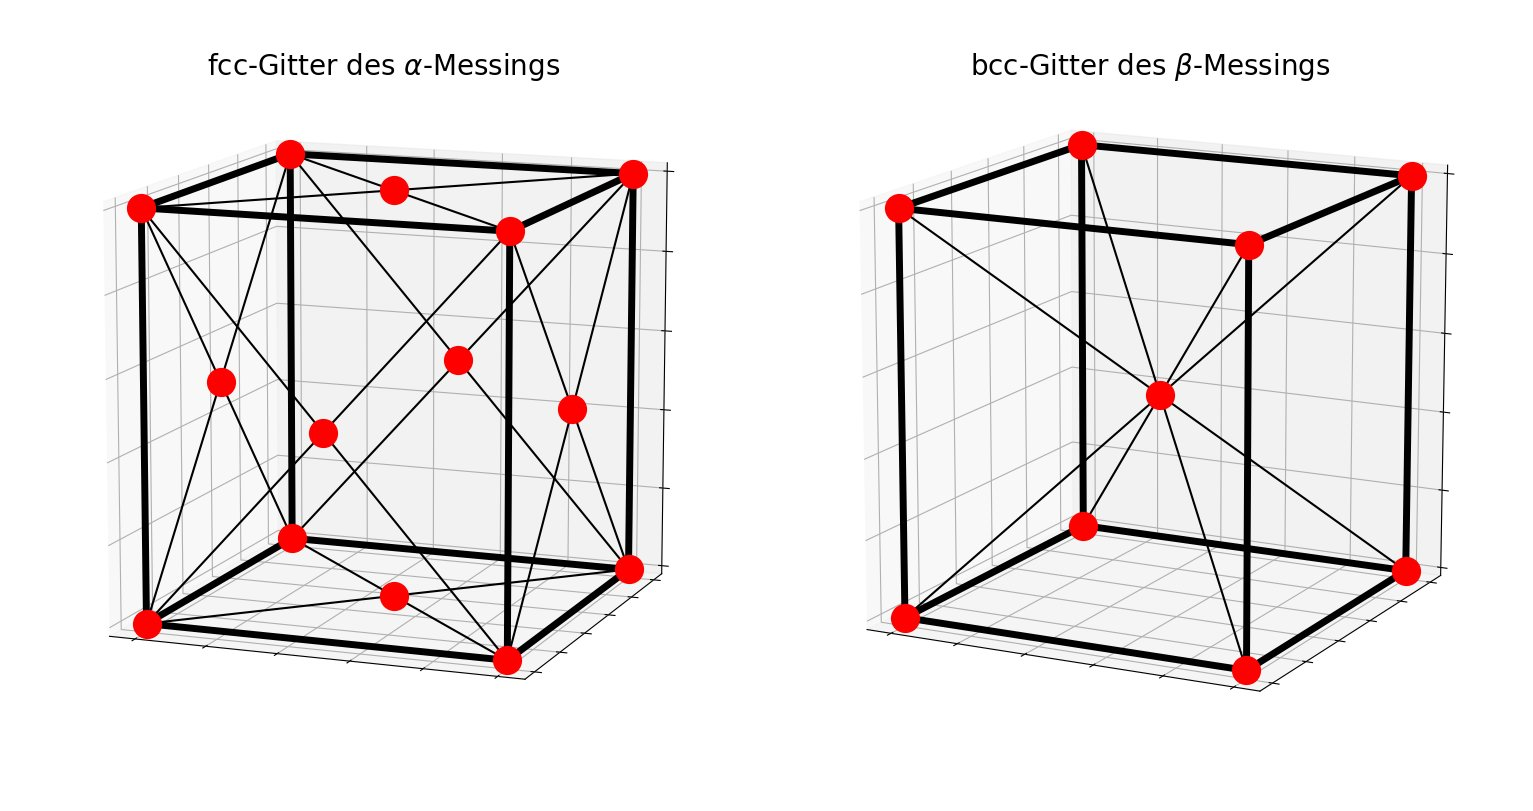
\includegraphics[width = \textwidth]{alpha_und_beta_Messing_Gitter.jpg}
\caption{Darstellung der Kristallstrukturen von \(\alpha\)- und \(\beta\)-Messing}
\end{figure} \\
\underline{\(\alpha\)-Messing:} \\\\
Beim \(\alpha\)-Messing handelt es sich um einen Mischkristall aus durchschnittlich 38 Atom-
prozent Zink und entsprechend 62 Atomprozent Kupfer. Die \(\alpha\)-Mischkristalle bilden ein
fcc-Gitter mit einer Gitterkonstanten von \(a_{\alpha} = 3.70 \text{\r A}\). Das fcc-Gitter enthält vier Atome pro Elementarzelle. Teilt man die Atommassen von Kupfer und Zink prozentual gemäß
obiger Zusammensetzung auf die vier Atome auf, kann man die Gesamtmasse der Elementarzelle berechnen:
\[m_{\mathrm{ges}} = 4\cdot (0.38\cdot m_{\mathrm{Zn}} + 0.62 \cdot m_{\mathrm{Cu}}) = 4.2659 \cdot 10^{-25} \ \mathrm{kg}\]
Das Gesamtvolumen der Einheitszelle ist gerade das Volumen des Würfels mit der Kantenlänge \(a_{\mathrm{\alpha}}\) , also:
\[V_{\mathrm{ges}} = a_{\alpha}^3 = \left(3.7\cdot 10^{-10} \ \mathrm{m}\right)^3 = 5.0653\cdot 10^{-29} \mathrm{m}^3\]
Die Dichte lässt sich dann leicht errechnen:
\[\underline{\underline{\rho_{\alpha} =  }} \frac{m_{\mathrm{ges}}}{V_{\mathrm{ges}}} = \frac{4.2659 \cdot 10^{-25} \ \mathrm{kg}}{5.0653\cdot 10^{-29} \mathrm{m}^3} = 8421.81 \frac{\mathrm{kg}}{\mathrm{m}^3} \underline{\underline{= 8.4218 \frac{\mathrm{g}}{\mathrm{cm}^3}}}\]
\underline{\(\beta\)-Messing:} \\\\
Beim \(\beta\)-Messing handelt es sich um einen Mischkristall aus durchschnittlich 44.3 Atom-
prozent Zink und entsprechend 55.7 Atomprozent Kupfer. Die \(\beta\)-Mischkristalle bilden ein
bcc-Gitter mit einer Gitterkonstanten von \(a_{\beta} = 2.94 \text{\r A}\). Das bcc-Gitter enthält zwei Atome pro Elementarzelle. Teilt man die Atommassen von Kupfer und Zink prozentual gemäß
obiger Zusammensetzung auf die zwei Atome auf, kann man die Gesamtmasse der Elementarzelle berechnen:
\[m_{\mathrm{ges}} = 2\cdot (0.443\cdot m_{\mathrm{Zn}} + 0.557 \cdot m_{\mathrm{Cu}}) = 2.1368 \cdot 10^{-25} \ \mathrm{kg}\]
Das Gesamtvolumen der Einheitszelle ist gerade das Volumen des Würfels mit der Kantenlänge \(a_{\mathrm{\beta}}\) , also:
\[V_{\mathrm{ges}} = a_{\beta}^3 = \left(2.94\cdot 10^{-10} \ \mathrm{m}\right)^3 = 2.5412\cdot 10^{-29} \mathrm{m}^3\]
Die Dichte lässt sich dann leicht errechnen:
\[\underline{\underline{\rho_{\beta} =  }} \frac{m_{\mathrm{ges}}}{V_{\mathrm{ges}}} = \frac{2.1368 \cdot 10^{-25} \ \mathrm{kg}}{2.5412\cdot 10^{-29} \mathrm{m}^3} = 8408.63 \frac{\mathrm{kg}}{\mathrm{m}^3} \underline{\underline{= 8.4086 \frac{\mathrm{g}}{\mathrm{cm}^3}}}\]
Die Dichten sind beide mit ein paar Stellen mehr als üblich angegeben, da mit diesen
Werten noch weiter gerechnet wird und somit Rundungsfehler vermieden werden. Ideale
Kristalle von \(\alpha\)- und \(\beta\)-Messing haben eine sehr ähnliche aber nicht ganz gleiche Dichte.
Man würde intuitiv vielleicht eine stärkere Abweichung erwarten, weil die Raumerfüllung
in einem fcc-Gitter bei etwa \(74 \%\) liegt; in einem bcc-Gitter dagegen nur bei etwa \(68 \% \).
Man muss allerdings berücksichtigen, dass die \(\beta\)-Phase einen signifikant höheren Zinkgehalt hat und Zink eine größere Atommasse hat als Kupfer. Außerdem ist die Elementarzelle des \(\beta\)-Messings etwas kleiner als die vom \(\alpha\)-Messing. Infolge dessen unterscheiden
sich die Dichten nicht so stark.
Diese Werte sind trotzdem nur idealisierte Dichten, da in jedem realen Kristall einerseits
Gitterfehler auftreten und andererseits auch die Kupfer- und Zinkgehalte nur Mittelwerte sind: Beispielsweise haben nicht alle \(\alpha\)-Mischkristalle den gleichen Zinkgehalt, weil sich
während der Kristallbildung der Kupfer- und Zinkgehalt der Schmelze kontinuierlich ändert. Entsprechendes gilt für \(\beta\)-Messing. Ausnahmen bilden eutektisch entstandene
Verbindungen mit definierter Zusammensetzung.
 % Bibliographie/Literaturverzeichnis
    \begin{thebibliography}{9}
    \bibitem{gitterfehler}
    \emph{Gitterfehler},
    \url{https://de.wikipedia.org/wiki/Gitterfehler#Nulldimensionale_Gitterfehler},
    9.\,Dez.~2019.
    \bibitem{wiki:Praktischer_Strahlenschutz}
    \emph{Schematische Darstellung von Stufenversetzungen (2D)},
    \url{https://de.wikipedia.org/wiki/Versetzung_(Materialwissenschaft)#/media/Datei:Versetzung_im_2D-Kristall.svg},
    12.\,Dez.~2019.
 \bibitem{gitterfehler}
    \emph{Schematische Darstellung von Stufenversetzungen (3D)},
    \url{https://de.wikipedia.org/wiki/Versetzung_(Materialwissenschaft)#/media/Datei:Dislocation_edge_d2.svgr},
    12.\,Dez.~2019.
\bibitem{gitterfehler}
    \emph{Schematische Darstellung von Klein- bzw- Großwinkelkorngrenzen},
    \url{https://docplayer.org/71200148-Technische-universitaet-graz.html},
    12.\,Dez.~2019.
\bibitem{Atommassen}
    \emph{Formelsammlung bis zum Abitur - Formeln Tabellen Daten, Dr.Lutz Engelmann u.A.,
Duden Paetec Schulbuchverlag},
    \end{thebibliography}

% ----- BEISPIELTEXT ENDE -----

\end{document}